% \documentclass[oneside]{report}
\documentclass[twoside,final,12pt,a4paper]{extreport}
\usepackage[T2A]{fontenc}


\usepackage{algorithm}
\usepackage{algpseudocode} %pseudo code



%%% Flowchart%%%
\usepackage{tikz} 
\usetikzlibrary{shapes.geometric, arrows}
\tikzstyle{startstop} = [rectangle, rounded corners, 
minimum width=3cm, 
minimum height=1cm,
text centered, 
draw=black, 
fill=red!30]

\tikzstyle{io} = [trapezium, 
trapezium stretches=true, % A later addition
trapezium left angle=70, 
trapezium right angle=110, 
minimum width=3cm, 
minimum height=1cm, text centered, 
draw=black, fill=blue!30]

\tikzstyle{process} = [rectangle, 
minimum width=3cm, 
minimum height=1cm, 
text centered, 
text width=3cm, 
draw=black, 
fill=orange!30]

\tikzstyle{decision} = [diamond, 
minimum width=3cm, 
minimum height=1cm, 
text centered, 
draw=black, 
fill=green!30]
\tikzstyle{arrow} = [thick,->,>=stealth]

%%% End Flowchart%%%


%%% Code display%%%%

\usepackage{xcolor}
\usepackage{listings}

% Define a light gray background color
\definecolor{lightgray}{rgb}{0.95,0.95,0.95}

\lstset{
  backgroundcolor=\color{lightgray},   % Gray box
  basicstyle=\ttfamily\small,          % Code font
  keywordstyle=\color{blue},           % Blue keywords
  commentstyle=\color{black},          % Black comments
  stringstyle=\color{blue},            % Blue strings
  showstringspaces=false,
  frame=single                         % Box border
}
%%%%%%%%%

\usepackage{vmargin}
\setpapersize{A4}
\setmarginsrb{2.5cm}{2cm}{2cm}{2cm}{0pt}{10mm}{0pt}{13mm}
\usepackage{setspace}
\sloppy
\setstretch{1.5}
\widowpenalty=10000
\clubpenalty=10000
\usepackage{indentfirst}
\parindent=1.25cm

%%%%% ADDED TO SUPPORT TT BOLD FACES %%%%
\DeclareFontShape{OT1}{cmtt}{bx}{n}{<5><6><7><8><9><10><10.95><12><14.4><17.28><20.74><24.88>cmttb10}{}
\renewcommand{\ttdefault}{pcr}
%%%%% END %%%%%%%%%%%%%%%%%%%%%%%%%%%%%%% 
\usepackage{atbegshi,picture}
\AtBeginShipout{\AtBeginShipoutUpperLeft{%
  \put(\dimexpr\paperwidth-1cm\relax,-1.5cm){\makebox[0pt][r]{
\includegraphics[width=3cm]{figs/CamTech-logo-wide.jpg}}}%
}}


\usepackage[english]{babel}
\usepackage[backend=biber,style=ieee,autocite=inline]{biblatex}
\bibliography{ref.bib}
\DefineBibliographyStrings{english}{%
  bibliography = {References},}
\usepackage{blindtext}
\usepackage{pdfpages}
\newenvironment{bottompar}{\par\vspace*{\fill}}{\clearpage}
\usepackage{amsmath,amsfonts}

\usepackage{amsthm}
\newtheorem{theorem}{Theorem}
\newtheorem{corollary}{Corollary}
\newtheorem{lemma}{Lemma}
\newtheorem{proposition}{Proposition}
\theoremstyle{definition}
\newtheorem{definition}{Definition}
\theoremstyle{remark}
\newtheorem*{remark}{Remark}
\theoremstyle{remark}
\newtheorem*{example}{Example}


\usepackage{float}
\usepackage{graphicx}
\graphicspath{{figs/}} %path to images
\usepackage{array}
\usepackage{multirow,array}
\usepackage{caption}
\usepackage{subcaption}
\usepackage{hyperref}
\usepackage{paralist}
\usepackage{listings}
\usepackage{zed-csp}
\usepackage{fancyhdr}
\usepackage{csquotes}
\usepackage{color}

\usepackage{upgreek} 
\usepackage{bm}
\usepackage{hyperref}
\usepackage{setspace}
\usepackage{booktabs}
\usepackage{multirow}
\usepackage{longtable}
\usepackage[font=singlespacing, labelfont=bf]{caption}

%Hints
\newcommand\pic[1]{(Fig. \ref{#1})} %Ref on figure
\newcommand\tab[1]{(Tab. \ref{#1})} %Ref on table


\usepackage{enumitem}
\newlist{inlinelist}{enumerate*}{1}
\setlist*[inlinelist,1]{%
  label=(\arabic*),
}

\fancypagestyle{noheaderfooter}{
  \fancyhf{}  % clear all header and footer fields
  \renewcommand{\headrulewidth}{0pt}
  \renewcommand{\footrulewidth}{0pt}
}



\pagestyle{fancyplain}

% remember section title
\renewcommand{\chaptermark}[1]%
	{\markboth{\chaptername~\thechapter~--~#1}{}}

% subsection number and title
\renewcommand{\sectionmark}[1]%
	{\markright{\thesection\ #1}}

\rhead[\fancyplain{}{\bf\leftmark}]%
      {\fancyplain{}{\bf\thepage}}
\lhead[\fancyplain{}{\bf\thepage}]%
      {\fancyplain{}{\bf\rightmark}}
\cfoot{} %bfseries


\newcommand{\dedication}[1]
   {\thispagestyle{empty}
     
   \begin{flushleft}\raggedleft #1\end{flushleft}
}

\begin{document}

% ========== FRONT MATTER ==========
% --- Title Page ---
\begin{titlepage}
    \centering

    
\includegraphics[width=13cm]{figs/CamTech-logo-wide.jpg}
    \vspace{0.5cm}

    {\Large\bfseries Cambodia University of Technology and Science}\\[1cm]

    \vspace*{7cm}
    {\large\bfseries Reaksmey Eb}\\[1cm]

    \vspace*{4cm}
    {\Large A Thesis Submitted in Partial Fulfillment of the Requirements for the Degree of}\\[0.5cm]
    {\large\bfseries Bachelor's Degree in Cybersecurity}\\[2cm]
\end{titlepage}

\newpage
\thispagestyle{empty}

\begin{center}

 {\Large\bfseries Cambodia University of Technology and Science}\\[0.25 cm]
    {\large\bfseries Faculty of Engineering}\\[4 cm]

    {\huge\bfseries Security Implementation for Guarantee of Payment System}\\[2cm]


    {\Large By}\\[0.5cm]
    {\Large\bfseries Reaksmey Eb}\\[0.5cm]
    {\Large (ID: 6023010017)}\\[3cm]
\end{center}
    \hspace*{2cm}{\Large Supervisor\hspace*{0.85cm}: Dr. Engelking Elias Jacob}\\[0.5cm]
    \hspace*{2cm}{\Large Mentor\hspace*{2cm}: Mr. Makara Long}\\[2.5cm]
\begin{center}
    {\large August, 2025 }\\

    {\large Phnom Penh, Cambodia}

    \vspace*{\fill} % Push to bottom

\end{center}

\thispagestyle{empty}

\begin{center}
    {\huge\bfseries Declaration of Originality}
\end{center}
\vspace{1 cm}
I, \textbf{Reaksmey Eb}, hereby declare that this thesis, titled \textbf{``Security Implementation for Guarantee of Payment System''}, submitted in partial fulfillment of the requirements for the degree of Bachelor of \textbf{Cybersecurity Engineering} at the Cambodia University of Technology and Science, is my own original work. This work was carried out during my industrial placement at \textbf{Intercare Hospital} from \textbf{March 5th, 2026} to \textbf{September 4th, 2026}. All sources and references used were properly acknowledged and cited.
\vspace{3cm} % Space for signature


\noindent\rule{6cm}{0.4pt} \\[0.1cm]
Full name\hspace*{1.05cm}:  Reaksmey Eb \\
Date\hspace*{2cm}: 01, August 2026

% --- Third Page: Thesis Approval ---
\newpage
\thispagestyle{empty}

\begin{center}

    {\huge \textbf{Report Approval}} \\[1.5cm]

    \begin{minipage}{0.9\textwidth}
    \onehalfspacing
    This report, titled ``\textbf{Security Implementation for Guarantee of Payment System}'', submitted by \textbf{Reaksmey Eb} (ID: \textbf{6023010017}), has been approved by the following members of the examination committee as a partial fulfillment of the requirements for the degree of \textbf{Bachelor degree in Cybersecurity Engineering} at the \textbf{Cambodia University of Technology and Science}.
    \end{minipage}

    \vspace{1cm}


\begin{tabbing}
    \hspace{5cm} \= \hspace{6cm} \= \hspace{4cm} \kill
    \Large \textbf{Report Submission Approval} \> \> \\[0.5cm]
        \textbf{Supervisor\hspace{1.2cm}: Dr. Engelking Elias Jacob}  \> \>\underline{\hspace{4cm}}  \\
        (Head of Digital Health, Intercare Hospital) \\

        \textbf{Mentor: Mr. Makara Long}  \> \>\underline{\hspace{4cm}} \\
        (Lecturer, CamTech University)
\\
\vspace{0.2cm}
\\
   \Large \textbf{Examination Committees Mentor} \> \> \\[0.5cm]

    \textbf{Committee 01: [Name]}  \> \>\underline{\hspace{4cm}}  \\
    (Title, Institution) \\
    \textbf{Committee 02: [Name]}  \> \>\underline{\hspace{4cm}}  \\
    (Title, Institution) \\
    \textbf{Committee 03: [Name]}  \> \>\underline{\hspace{4cm}}  \\
    (Title, Institution) \\
    \textbf{Committee Chair: [Name]}  \> \>\underline{\hspace{4cm}} \\
    (Title, Institution)
\\
\vspace{0.2cm}
\\
    \Large \textbf{Acknowledged by} \> \> \\[0.5cm]

    \textbf{Name, Title:} \>  \> \underline{\hspace{4cm}}
    \\
    \textbf{Date of Approval:} \>  \> \underline{\hspace{4cm}}\\
\end{tabbing}

\end{center}

% --- Acknowledgements ---

\newpage
\thispagestyle{empty}

 \begin{center}
     {\huge \textbf{Acknowledgements}} \\[1.5cm]
 \end{center}

I would like to express my sincere gratitude to CamTech University for the opportunity to undertake this placement, and for its support throughout, from the very start of the process to its completion.

My sincere thanks go to Intercare Hospital for hosting this placement within such a professional and welcoming environment.

I wish to express my deepest gratitude to my supervisor, Dr. Elias. You placed your trust in me even though I had no real experience and lacked the skills this work demanded. You stood by me through every situation, followed up when I needed it, and listened patiently even on my hardest days, always ready to talk things through with me. You pushed me further than I ever thought I could go, and helped me grow into someone I wasn't six months ago. This time under your guidance has been truly precious to me.

I would like to convey my sincere gratitude to my mentor, Loukru Makara. Your steady direction, especially at moments when I was uncertain how to proceed, was invaluable throughout this project. I appreciate the patience and encouragement you offered at every stage.

I am sincerely grateful to Dr. Ebner, Deputy CEO of Intercare, whose contribution made this project possible to carry through in many ways.

I extend special appreciation to the IT team, Bong Udom, Bong Chantha, and Bong Savda, who formed the backbone of this project's technical work, offering ideas, consultation, and support at every step.

I extend my sincere appreciation to Mrs. Debbie, Mrs. Riza, Bong Kimheng, Dr. Denny, Dr. Justyna, and Dr. Visoth, for your support and the time you spent answering our endless questions along the way.

To my dear friends on the GOP-MVP project, Rith (Soputhearith), who led development and communication, and Chamrath, who was responsible for data organisation and the ANZER adaptation, I am grateful for your collaboration and dedication throughout this project. This project would not have succeeded without the work each of you contributed, and I value the effort we put in together.

Lastly, I am immensely grateful to my family for your continued support throughout this placement. Your patience and encouragement, even without always knowing the details of the work, meant more than you may realise.

Finally, I extend my heartfelt thanks to everyone else who contributed to this project in ways not individually named here. Your assistance is sincerely appreciated.

% --- Abstract ---

\newpage
\thispagestyle{empty}

 \begin{center}
     {\huge \textbf{Abstract}} \\[1.5cm]
 \end{center}

Intercare Hospital processes insurance Guarantee of Payment (GOP) requests by hand, which causes delays, errors, and inconsistency. Automating this work places patient clinical data and hospital pricing in a single system used by five staff roles with different responsibilities. This study designed, implemented, and verified the security of that system, covering identity management, access control, audit logging, and vulnerability assessment. The NIST Cybersecurity Framework 2.0 structured the work, with STRIDE used for threat modelling and the 2021 edition of the OWASP Top 10 for code review. Keycloak was selected over a cloud service because the hospital required hosting on its own servers. Access control combined role-based (RBAC) and attribute-based (ABAC) rules across forty-two defined actions, supported by an append-only audit log. Verification used both automated scanning and manual role-by-role testing of the running system. Static analysis with Semgrep covered 356 files and produced 15 findings. None concerned access control. Manual role-by-role testing of the same system in the same period produced 47 tracked findings, of which 23 were access-control findings. Most were fixed before deployment, and the rest were recorded as deferred decisions. Permissions were found to depend on three factors together: the user's role, their assignment to a case, and how far that case had progressed through the workflow. These findings indicate that automated scanning alone cannot verify authorisation logic, because such rules depend on organisational policy rather than on code structure. They also show that access control in clinical workflows must depend on the state of a case, not on the user's role alone.
\\
\textbf{Keywords:} access control, role-based access control (RBAC), attribute-based access control (ABAC), Keycloak, healthcare information systems, security testing


\tableofcontents
\listoftables
\listoffigures




\newpage
\chapter{Introduction}
\label{chap:intro}
\chaptermark{Introduction}

This chapter introduces the setting of the project and the problem it addresses. It describes how Guarantee of Payment requests were handled at Intercare Hospital before the system was built. It then gives an overview of the hospital and the project, states the objectives of this thesis, and outlines the structure of the chapters that follow.

\section{Background of the Study}
\label{sec:intro-background}

Hospitals and insurance companies work together through a process known as Guarantee of Payment (GOP). Before a planned admission, the hospital asks the insurer to confirm in writing that it will cover the cost of treatment, so the patient can be treated without paying up front. The request is not a single document but a package: patient details, a clinical description of the planned procedure, statements from the treating doctors, and an itemised cost estimate. Because insurers set their own forms and required fields, assembling that package is manual work that falls on hospital staff, and the effort grows with the number of insurers a hospital works with.

At Intercare Hospital in Phnom Penh, this process was carried out manually, and a single request could pass through four departments before it reached the insurer. The result was slow, inconsistent, and tiring for the people doing it. Chapter \ref{chap:ps} describes that process in detail.

Automating this process removes much of that effort, but it also changes where the risk sits. Information that once lived on paper in a single office now sits in a database that many people can reach across the hospital network. Decisions that were previously made in person, such as who is allowed to confirm a cost or approve a clinical statement, become rules written into software. A GOP request contains both clinical information about a patient and a financial commitment on behalf of the hospital, so a mistake in those rules is not only a privacy problem but a financial one.

Security therefore could not be treated as something added after the system worked. It covers more than one question: who is allowed into the system, what each person may do once inside, what record is kept of what they did, and whether the software and servers the system runs on are themselves safe. These questions had to be answered alongside the workflow rather than after it. This thesis describes the requirements that were identified, the security that was designed and built to meet them, and how the result was tested and revised.

\section{Company Overview}
\label{sec:intro-company}

Intercare Hospital is a private healthcare provider in Phnom Penh, Cambodia, based at the Olympia Medical Hub Building on Street 161, Veal Vong, 7 Makara. The hospital's stated aim is to become the most trusted healthcare provider in Cambodia, with values organised under a framework called I-CARE, covering innovation, compassion, accountability, responsiveness and empowerment \cite{intercare}.

The hospital opened in 2020 as a general practice clinic and has added services each year since: laboratory and imaging in 2021, maternity, inpatient and emergency care in 2022, and operating theatre services, physiotherapy and a visa health check centre in 2023. Paediatrics, a child wellbeing centre and a set of community clinics under the Intercare Express name followed, with a medical centre in Siem Reap planned \cite{intercare}.

The hospital employs more than two hundred medical professionals, Cambodian and international, representing over twenty nationalities, and treats Cambodian families, expatriates, company employees and travellers. Care is provided in partnership with more than forty insurance providers, which makes the Guarantee of Payment process a routine part of daily work rather than an occasional task \cite{intercare}.

\section{Project Overview}
\label{sec:intro-project}

This project was carried out within the hospital's Digital Health department, which is responsible for the systems that support clinical and administrative work. The aim was to replace the manual cost estimation and Guarantee of Payment process with a web-based system, so that a request could be prepared, reviewed and sent from one place instead of being assembled by hand across several departments.

The wider effort is planned in three phases. This project delivers Phase 1, built over six months as the internal foundation that later phases can extend without being rebuilt. Phase 1 covers the hospital's own side of the workflow: creating a case from patient and encounter data, building a cost estimate, generating the GOP request and its document output, tracking its status through approval, rejection or revision, and keeping an audit trail. The system does not connect to insurer systems. Finance reviews each case and sends the request from within the system; nothing goes out automatically. The insurer's reply arrives in a staff Outlook mailbox rather than in the system, so Finance records the answer by hand, and a case needing revision is corrected and sent again by the same path. Claims generation and submission belong to later phases. The system's data model follows the HL7 Fast Healthcare Interoperability Resources (FHIR) standard, which shaped several of the security decisions described later. At the time of writing, some parts of this workflow were complete and working, while others were still being finished.

The system was built by a team of three students on industry placement, each from a different major: software engineering, data science and artificial intelligence, and cybersecurity. My major is cybersecurity, and I was responsible for the security of the system. That covered working out what needed to be protected, designing and building the controls to protect it, and testing whether they held. This thesis describes that security work.

The system was built for internal use within the hospital rather than for public access, and is hosted on the hospital's own servers rather than in the cloud. This decision shaped much of the security design, as the responsibility for protecting the system and the environment it runs on stays with the hospital.

\section{Research Objectives}
\label{sec:intro-objectives}

The general objective of this work was to build security into the Guarantee of Payment system as it was developed, rather than adding it once the system was working. The specific objectives were as follows.

\begin{enumerate}
    \item To identify what the system needs to protect, and to establish the security requirements of the workflow, including the separations between roles that already exist in hospital practice.
    \item To select security standards suitable for a small internal health system that can also be extended as the system grows, and to state how far each one is applied.
    \item To design and implement the security of the system: signing in, what each user may do, how their actions are recorded, and the security of the software the system runs on.
    \item To evaluate the security before deployment, using manual testing, automated scanning, and a separate assessment against the OWASP Application Security Verification Standard, and to record what was found.
    \item To compare what each method detected, and to discuss what that means for verifying access control in systems of this kind.
\end{enumerate}

\section{Thesis Structure}
\label{sec:intro-structure}

This thesis is organised into seven chapters.

\begin{itemize}
    \item Chapter \ref{chap:intro} introduces the setting, the hospital, the project, and the objectives of this work.
    \item Chapter \ref{chap:ps} describes the problem: how Guarantee of Payment requests were handled manually, what that cost the hospital, and which part of it this project addresses.
    \item Chapter \ref{chap:lr} reviews existing work on access control models, security standards for health information systems, threat modelling, and how access control is verified.
    \item Chapter \ref{chap:met} sets out the method, including the frameworks applied and how far each one was used.
    \item Chapter \ref{chap:impl} describes what was built: how users are identified, the access control model, the audit trail, and the security of the deployment.
    \item Chapter \ref{chap:result} reports what the verification produced and discusses what those results mean.
    \item Chapter \ref{chap:conclusion} covers the difficulties encountered, the conclusions drawn, and the work that remains.
\end{itemize}

\chapter{Problem Statement}
\label{chap:ps}
\chaptermark{Problem Statement}

This chapter sets out the problem the project addresses. It describes how Guarantee of Payment requests were handled before the system was built, what that process cost the hospital, which part of it this thesis is concerned with, and what the problem amounts to when stated in short.

\section{Background of the Problem}
\label{sec:ps-background}

A Guarantee of Payment request is assembled from parts held by different people. The patient's identity and insurance details sit with the front desk, the clinical description comes from the surgeon, a separate assessment comes from the anaesthetist, and Finance builds the itemised cost from the hospital's own pricing. Each insurer sets its own form and required fields, so the same case may be presented differently depending on who is being asked to pay.

At Intercare Hospital this was done on paper, and the paper travelled. The surgeon and anaesthetist completed their parts and handed the file to the Surgical Coordinator, who checked it for missing information. Where something was missing, the Coordinator went back to the doctor concerned, who either supplied it themselves or gave permission for the Coordinator to enter it on their behalf. Once complete, the file went to Finance for costing, returned to the Coordinator for the patient's acknowledgement, and if the patient agreed went back to Finance to be sent to the insurer. If the patient declined, the case ended there.

The paper file was the control. Only the person holding it could act in that case. Nothing moved forward unless someone carried it, and an incomplete case went back to the doctor. The order of the work, the point at which each group's part ended, and the separation between the clinical and financial sides were all carried by the movement of that paper. None of it was written down as a rule, because none of it needed to be.

Automating this is not just moving the same process onto a screen. Once the file becomes a database record, everyone can reach it at any time, and the sequence the paper enforced no longer exists.

The new system removes the Coordinator as a required stop. The doctors now pass the case to Finance directly. The Coordinator now only watches progress; editing another role's part of a case is no longer something the Coordinator does. This was not the original plan. Early in the work, the Coordinator kept a narrow edit right carried over directly from paper: the ability to adjust a case's pricing after Finance had verified it, on the understanding that the change had been agreed by phone or in person first, with only the audit log to show who made it. The system had no way to check that the conversation actually happened, so the edit was allowed and simply recorded. That exception was closed before the work finished. The Coordinator's editing rights were narrowed to their own scope only, case priority and response-time targets, and the trust-based allowance was removed rather than kept.

\begin{figure}[H]
  \centering
  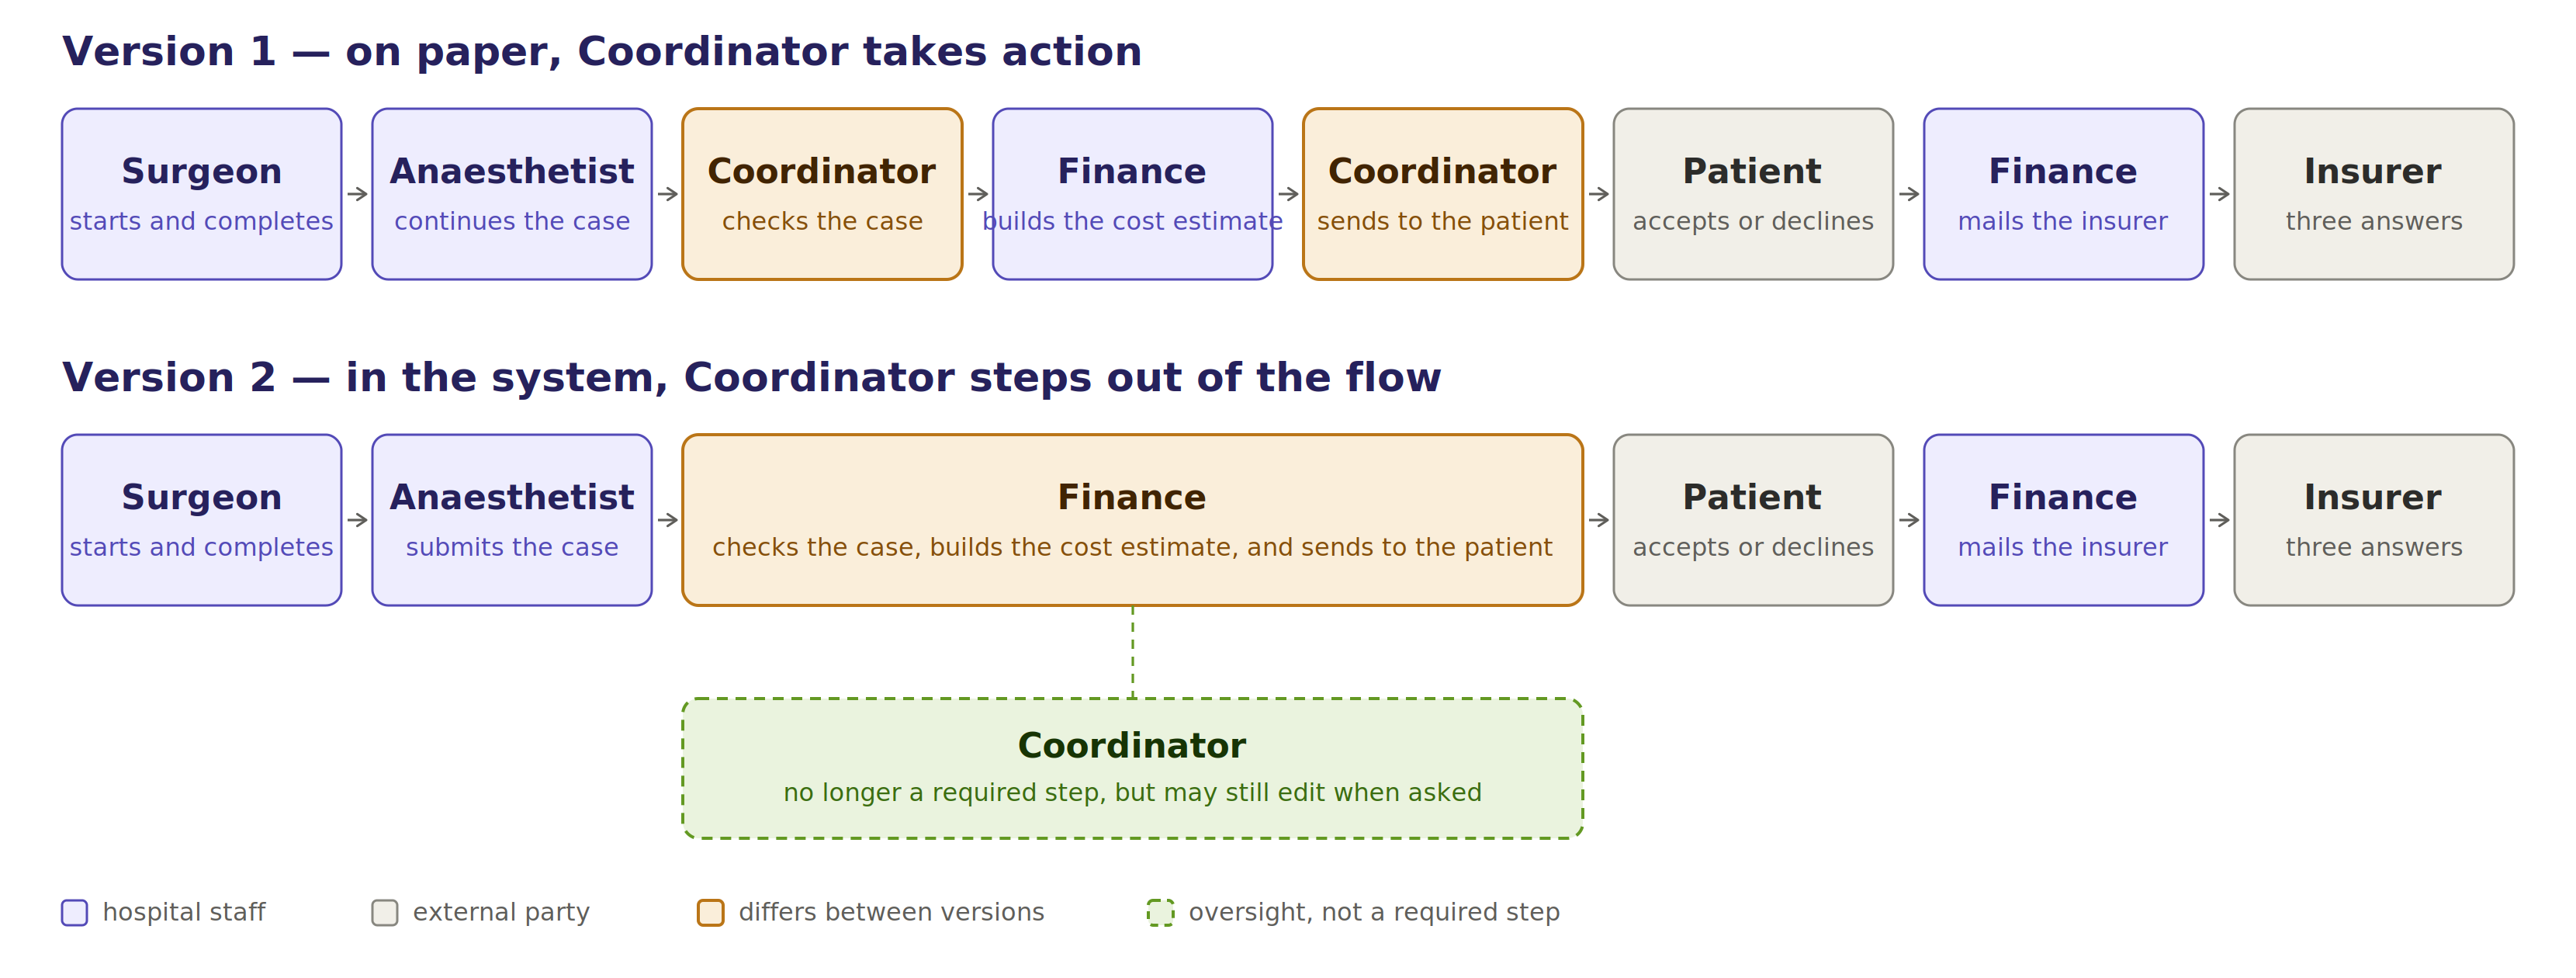
\includegraphics[width=\textwidth]{figs/Figure1-GOP-Process-Flow-Comparison.png}
  \caption{The GOP process on paper compared with the process in the system. Amber marks where the two differ. A patient who declines ends the case; where the insurer asks for changes, Finance revises the request and sends it again.}
  \label{fig:process-comparison}
\end{figure}

On paper, the Coordinator had to walk over and ask before changing a doctor's form. In software, nothing physical stops anyone. So each rule the paper enforced had to become one of two things. Most rules the code blocks outright: the surgeon and anaesthetist can no longer edit a case once it reaches Finance, and the system refuses the change. One rule briefly took the other path, allowed without a check and only logged, trusting that the real-world conversation had happened. That was the Coordinator's pricing edit described above, and it is the only example of that pattern found anywhere in the system. It did not stay that way for long: by the time this work finished, it had been closed and folded into the first kind of rule instead, so every rule the paper enforced is now enforced by code, with no trust-based exception left standing.

\section{Impact of the Problem}
\label{sec:ps-impact}

The manual process cost staff time. Preparing one request meant collecting information that already existed elsewhere. Staff walked between departments to get it, then typed the same patient details more than once as the file moved. A request passed through four departments before it left the hospital, and each hand-off waited on someone being free to receive it.

The clearest case was the handover to Finance. The surgeon and anaesthetist wrote their parts by hand, and Finance then re-entered all of it digitally, because both the patient consent form and the insurer's request had to be produced as documents. With each insurer setting its own format, the same handwritten case could be typed out in more than one layout.

The process also depended on people who are hard to reach. Finance and the Coordinator could not move a case forward until the surgeon and anaesthetist had entered their parts, and staff report that those parts were sometimes forgotten or supplied late. Chasing a doctor who is in theatre or between patients is not quick, so a case could sit waiting on one missing figure.

Order was also difficult to keep. With cases held as paper files, there was nothing to show which had been waiting longest or which needed attention first. Staff report that a case opened early could finish last, and that an emergency case could be delayed simply because the file was hard to find among the others. Nothing about a stack of paper tells you what is urgent.

Repetition also costs accuracy. Details typed a second or third time can be typed differently, a date entered as the fourth month rather than the third, for instance. The information the doctors supplied was correct; the copying was where it went wrong. A mismatch between the patient record, the clinical description and the cost is the kind of error an insurer returns rather than resolves. And because each insurer sets its own form, a missing field found late meant the request came back and the work was done again.

The paper carried its own record. The file showed who the doctors were, who handed it on, and when. That record existed as a by-product of being paper: a signature had to be written, a date entered, and a correction crossed out in view of whoever held the file next. Software keeps none of that by itself. A database shows the current value of a field, not who set it or what it was before. The record has to be built deliberately, or there is none.

\section{Scope of the Problem}
\label{sec:ps-scope}

Not all of the problems described above are addressed here. The security work covers signing in, what each user may do, how their actions are recorded, and the security of the software the system runs on. It also covers the administration screens themselves: the interface for enabling and disabling accounts, and the view onto the audit trail. The application logic, the integration with the hospital information system, and the database design were the work of my teammates, and appear in this thesis only where a security decision depends on them.

Because the system is not internet-facing, this phase focused primarily on authenticated internal users, compromised internal accounts, and misuse of legitimate access, while recognising that external compromise could still occur indirectly through the hospital network, for instance through a stolen credential, a compromised endpoint, or lateral movement from elsewhere on the network. Two checks were outstanding at the time this scope was set: a penetration test by the hospital's IT Security Division, and a review of the container settings against the Center for Internet Security (CIS) Docker Benchmark. The first has since been carried out, by Canadia Bank (IT security department) together with the hospital's IT Security Division. The second, the container review, has also since been carried out by Canadia Bank (IT security department), though not confirmed as following the CIS Docker Benchmark specifically. Going live also required a signed non-disclosure agreement, hospital approval, and privacy safeguards, all agreed at the start of the project.

\section{Summary of the Problem}
\label{sec:ps-summary}

The manual Guarantee of Payment process was slow, repetitive and open to error. It did keep a record of who did what, but only because the paper carried signatures, dates and visible corrections.

Automating it removes the costs. It also removes two things that came free with the paper. The first is the physical route that quietly enforced the order of the work: who could act on a case, at what point their part ended, and where the clinical side stopped and the financial side began. The second is the record itself.

Software will not make people work in order, and it will not keep a history. You have to build both. Every rule must be written into the code. Every action must be saved on purpose. On paper, someone nearby might spot a mistake. In software, no one is nearby. If a rule is wrong, nothing catches it.

The question is not whether the process can be automated. It is whether the system can be trusted to let the right people do the right things. Answering it means listing every action the system allows, deciding the rule for each one, putting the check somewhere the user cannot get past, recording what happened, and then testing that it works.

\chapter{Literature Review}
\label{chap:lr}
\chaptermark{Literature Review}

This chapter reviews the existing work this project uses. The work covered the security of the system as a whole: signing in, what each user may do, how their actions are recorded, and the security of the software the system runs on. A systematic review of access control in electronic health record systems groups this field into identification, authentication, authorisation and accountability \cite{cobrado2024}, and those four categories match the strands of work described in Chapter \ref{chap:met}.

The review is weighted towards authorisation, because that is what most of this project's findings are about. Section \ref{sec:lr-rbac-abac} covers the models of authorisation and what each can express. Section \ref{sec:lr-standards} covers the standards that apply to health information systems, which between them address identification, authentication, transport and audit. Section \ref{sec:lr-threat} covers threat modelling. Section \ref{sec:lr-verification} covers how access control is verified, which is where the main result of this project lies.

\section{Access Control Models: RBAC and ABAC}
\label{sec:lr-rbac-abac}

Access control decides which users may do what, and to which records. Two models are treated as the classic approaches, and FHIR's security guidance describes both for health systems \cite{hl7fhir}. In role-based access control (RBAC), permissions are grouped into roles, each role describes a job function, and users are given roles. If a user's role holds the permission, access is granted \cite{hl7fhir}. Permissions follow the job rather than the person, which suits a hospital, where roles such as surgeon, anaesthetist and finance officer already exist before any software is written.

In attribute-based access control (ABAC), the decision is made from attributes and conditions rather than from roles alone. The National Institute of Standards and Technology (NIST) describes ABAC as a method in which authorisation is determined by evaluating attributes of the subject, attributes of the object, the requested operation, and in some cases the conditions of the environment, against rules that describe which operations a given set of attributes allows \cite{nist80162}. NIST places ABAC on a spectrum of logical access control that also includes access control lists and role-based access control, so it is a development of earlier approaches rather than a replacement for them \cite{nist80162}. The practical gain is that rules may refer to the record itself. ``A surgeon may create a case'' is a role rule. ``A surgeon may edit this case'' is not, because the answer depends on the case, who it is assigned to, not on the surgeon.

Both standards recognise that a decision may also depend on the circumstances of the request, and both make room for it in their models. NIST calls this environment conditions and lists it as one of the four inputs to a decision, alongside rules, subject attributes and object attributes \cite{nist80162}. FHIR uses the term transaction context and names, among its examples, the workflow state of the request \cite{hl7fhir}. The workflow position of a case is therefore recognised in both, though under different names and in different parts of the model.

Work on access control in health systems has followed the same direction. A systematic review of twenty studies on electronic health record systems found attribute-based access control to be the most common authorisation mechanism, and grouped the mechanisms proposed into identification, authentication, authorisation and accountability \cite{cobrado2024}. The review also names what the literature has not resolved: multi-factor authentication, emergency access, patient consent and accountability are identified as gaps, with accountability addressed by only two of the twenty studies. Others have combined the two models directly. Atlam and Yang propose a healthcare model integrating role-based categorisation with attribute-based control over user attributes and environmental factors, observing that models which allocate permissions by predetermined roles or policies adapt poorly to the changing circumstances of a working healthcare system \cite{atlam2025}.

The three inputs are not alternatives. Roles carry the decisions that follow the job, attributes carry those that depend on the individual record, and the case's position in the workflow carries those that depend on how far it has progressed. What neither standard describes is how they combine in practice, what it costs to enforce them consistently, or how such rules can be checked once built. Chapters \ref{chap:impl} and \ref{chap:result} report that.

\section{Security Standards for Health Information Systems}
\label{sec:lr-standards}

Health information systems carry data that is sensitive in ways ordinary business systems are not. FHIR's security guidance was the health-specific source used here. It is unusual in addressing implementation directly: it recommends OAuth for authenticating users, states that production data should be sent over TLS, describes how audit events should be recorded, and sets out how a server should respond when access is refused \cite{hl7fhir}.

No Cambodian standard exists for health information security that a hospital can adopt. The nearest domestic guidance is the National Bank of Cambodia's Technology and Cyber Risk Management Guidelines, issued in January 2026 \cite{nbc2026}. These apply to banks rather than hospitals, so this system is not subject to them. They are, however, the only Cambodian document setting out detailed security requirements for systems holding sensitive data, and the requirements used here concern the protection of that data rather than financial services.

The guidelines require role-based access control with least privilege, a maintained access control matrix, segregation of duties so that no single person can enter, authorise and complete a transaction, audit logs that record both successful and refused access and cannot be altered, encryption of data in transit and at rest, and vulnerability assessment using both automated tools and manual techniques \cite{nbc2026}. They also note that Cambodia's adoption of technology is outpacing its regulatory frameworks, and direct institutions to adopt recognised standards where no local regulation exists \cite{nbc2026}.

This project follows that direction. Two general frameworks were used alongside FHIR. The NIST Cybersecurity Framework organises security work into six functions, Govern, Identify, Protect, Detect, Respond and Recover, and was used to structure the phases of the project rather than as a control set implemented in full \cite{nistcsf2}. The Open Worldwide Application Security Project (OWASP) publishes a list of the ten most common categories of web application security risk, used here as the checklist for reviewing the code \cite{owasp2021}. Each source serves one purpose: FHIR gives health-specific implementation guidance, NIST SP 800-162 the access control model, the National Bank of Cambodia guidelines a domestic benchmark, the NIST Cybersecurity Framework a structure for the work, and the OWASP Top 10 a checklist for the code.

None of these covers the part that matters most for a workflow system. They describe how to authenticate users, how to protect data in transit, what kinds of flaws to look for, and how to organise the work. None states who in a particular hospital may perform a particular action on a particular case, because that depends on how that hospital divides responsibility. Those rules must be drawn from the workflow itself, and the standards give no method for doing so, nor for checking the result.

\section{Threat Modelling Approaches}
\label{sec:lr-threat}

Threat modelling is the practice of working out what could go wrong with a system, without testing it. It asks what someone might attempt against each part of a system, and what would follow if they succeeded. OWASP treats it as a design activity. Its category for insecure design calls for greater use of threat modelling in authentication, access control and business logic, and separates design flaws from implementation defects, on the grounds that a design flaw cannot be fixed by careful coding \cite{owasp2021}.

STRIDE is the most widely used method. It groups threats into six kinds \cite{stride}: spoofing, where someone acts as another user; tampering, where data is changed without permission; repudiation, where a user denies an action and no record contradicts them; information disclosure, where data reaches someone who should not see it; denial of service, where the system is made unavailable; and elevation of privilege, where a user gains rights they were not granted. Each part of a system is examined against all six.

The value of the method is coverage, not discovery. Working through six categories for every component makes it harder to miss a whole class of threat. What STRIDE does not do is say which threats matter most, or supply the rules that would prevent them. It can tell you a system may be vulnerable to tampering. It cannot tell you which staff member should lose the ability to edit a record once another department has reviewed it. That judgement comes from the workflow, not from the method.

Threat modelling is usually described as a design-time activity, carried out before a system is built. It can also be applied to a system that already exists. In that case it organises and classifies what is known, rather than predicting what has not yet been found. Chapter \ref{chap:met} describes which of these applies to this project.

\section{Automated and Manual Security Verification}
\label{sec:lr-verification}

Writing down who may do what is one task. Checking that the software actually does it is another. A rule table states what should happen, but it says nothing about what the code does. The two can disagree without anyone noticing, because when a system allows something it should have blocked, nothing appears to go wrong. Not every strand of this work presents the same difficulty. Dependency versions, container images and secrets left in a repository can each be checked by tools, because each has a recognisable form. Access control does not, which is why it is the strand this section concentrates on.

Automated tools are the usual first step, and their main difficulty is well documented. Sun, Xu and Su point out that access control rules are specific to each application \cite{sun2011}. Unlike an injection flaw, which looks much the same in any program, there is no general pattern for a tool to search for. The rules have to be supplied, and writing them by hand is slow and tends to produce rules that are missing, incomplete or wrong. Their own tool works around this by inferring the rules from the source code: it builds a list of the pages each role can open, compares those lists to find pages only some roles should reach, and then tests whether other users can reach them anyway.

Inferring the rules from code is where the method reaches its limit. Zhu and colleagues tested six open source applications and found that the assumptions built into earlier tools held those tools back \cite{zhu2015}. They tried a different approach, asking developers to supply the rules and turning those answers into patterns the tool could then apply. This found twenty vulnerabilities the automatic methods had missed. A survey published in 2024 reaches the same conclusion, comparing the methods available and listing the problems that remain unsolved \cite{anas2024}. The pattern across all three is that access control rules come from the organisation rather than from the code, and that a tool performs better once a person supplies them.

This is why automated analysis cannot be the whole of the work, and the guidance says as much. OWASP asks developers to write tests for access control \cite{owasp2021}. The National Bank of Cambodia's guidelines require both automated tools and manual techniques \cite{nbc2026}. Neither explains how to test permissions that change as a case moves from one stage to the next. Chapter \ref{chap:result} reports what each method found when both were used on the same system in the same period.

\chapter{Methodology}
\label{chap:met}
\chaptermark{Methodology}

This chapter describes how the security work was carried out. It covers how the work was organised, which frameworks and standards were applied and how far, the threat model, and the tools used.

\section{Research Design}
\label{sec:met-design}

I planned the security work in seven steps: planning and requirements, choosing tools, design, building, testing before deployment, deployment, and checking afterwards. These were grouped under the functions of the NIST Cybersecurity Framework 2.0, and Figure \ref{fig:seven-phases} shows them. Five were completed at the time this was written; deployment, carried out by a teammate, had not fully succeeded, and the checks that follow deployment had not begun. Deployment has since been completed, every fix verified locally during this work is now live on the hospital's server, though the post-deployment checks (Section \ref{sec:conc-future}) remain outstanding. The five phases that ran did not run once each in order. Every time I checked something, I found a reason to change a decision I had already made, so the design, the build and the testing each came round more than once. That is why I call the method build-and-check cycles. The seven steps say what I planned; the cycles say how it actually ran.

\begin{figure}[H]
  \centering
  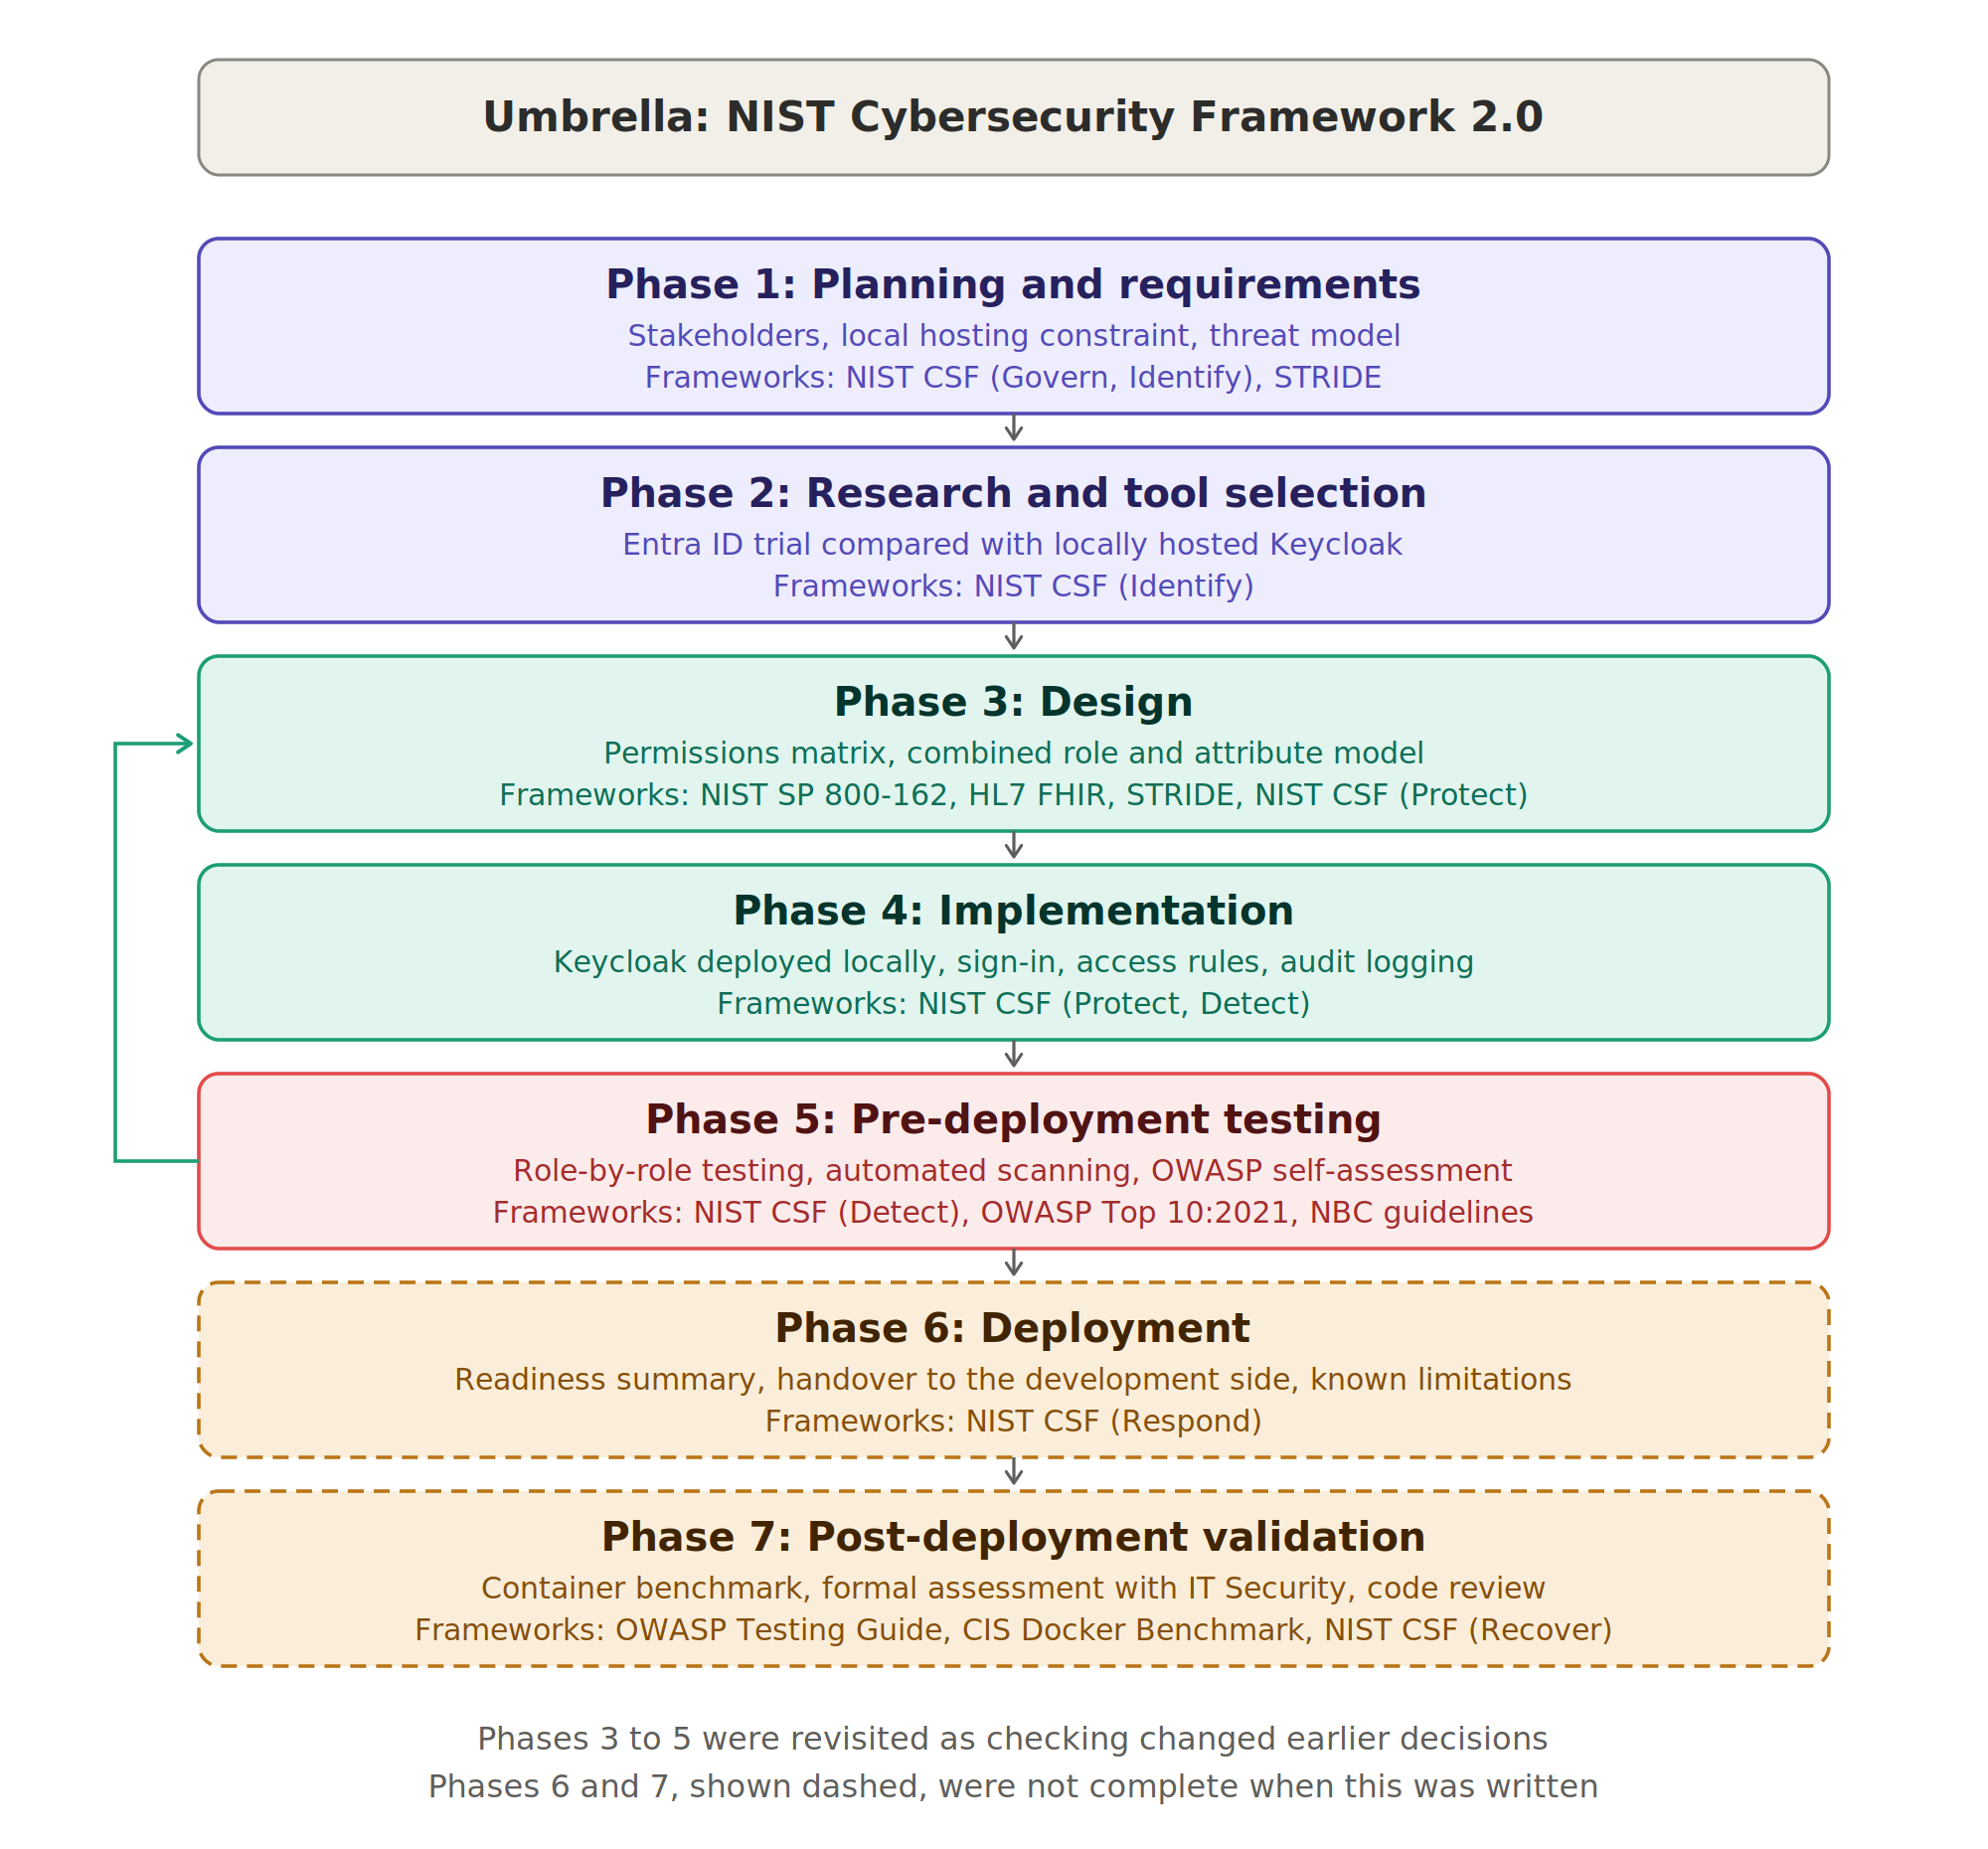
\includegraphics[width=\textwidth]{figs/Figure2-Seven-Phases.png}
  \caption{The seven phases of the security work, mapped to the functions of the NIST Cybersecurity Framework 2.0. Phases 3 to 5 were revisited as checking changed earlier decisions. Phases 6 and 7 were not complete at the time of writing.}
  \label{fig:seven-phases}
\end{figure}

The work covered four things: signing in, what each user may do, how their actions are recorded, and the security of the software the system runs on. Going round more than once mattered. I could not check the rules until I had written them, and I could not write them correctly until I had tested the system.

I did not begin from a written table. The code already existed, written by my teammate, so I started by reading it and writing down what it allowed each role to do. That gave the first version of the rules document. I then went through it against the workflow the team needed, adding rules and changing others, and writing down every difference I found. Some of those differences I could settle myself. Others needed the team to decide. A few are still open, because they depend on how staff want to work. Differences where the code was simply wrong were listed separately from differences where nobody had decided yet. Both lists are in the rules document. This review was the first of three checks.

The second check was manual testing, role by role, on the running system on my own machine. I signed in with one account for each of the five roles and followed a case from creation through to the insurer's decision. Where the system behaved differently from the rules, I recorded a finding. I then either fixed it, left it with a written reason, or closed it because the system was right and the rule was wrong.

The third check used automated tools on the same version of the code, in the same period: one for the packages the system depends on, one for the container images, one for passwords left in files, and one for the team's own code. I ran the scanners and the manual testing on the same version at the same time, on purpose. It means the two sets of findings can be compared directly, rather than across a version that had changed in between.

A fourth pattern ran alongside these three. I passed changes to the teammate handling deployment, and when a problem turned out to be on the security side, it was reported back to me, I corrected it, and passed it on again. Some problems only appeared once the system was installed, and those reached me through those reports rather than through my own testing.

Each cycle produced documents as well as code changes: the access control rules table, a record of each scan, an assessment against all ten OWASP categories, and a summary of what remained open and who owned it. I wrote these while working, not afterwards, and they are where the numbers in Chapter \ref{chap:result} come from.

I used AI tooling to help write and investigate code, under my direction. What to examine, whether a finding was real, and what to fix or defer were my decisions. I checked what the tooling reported against the running system before accepting it, and several reports turned out to be wrong.

\section{Frameworks and Standards Applied}
\label{sec:met-frameworks}

I applied frameworks selectively rather than in full. Table \ref{tab:frameworks} states which version I used and how far each one was applied, including the two that were planned but not carried out in this phase. Where a newer version has been published since this work was done, the version listed is the one that was current at the time, and re-assessment against the newer version is recorded in Section \ref{sec:conc-future}.

\begin{table}[H]
\centering
\caption{Frameworks and standards used, and how far each was applied.}
\label{tab:frameworks}
\begin{tabular}{|p{4cm}|p{2cm}|p{7.9cm}|}
\hline
\textbf{Framework} & \textbf{Version} & \textbf{Extent of application} \\
\hline
NIST Cybersecurity Framework & 2.0 (2024) & Six functions used to organise the work; control set not implemented \\
\hline
HL7 FHIR & R5 & Security section only \\
\hline
NIST SP 800-162 & 2014 & Definition and model of attribute-based access control \\
\hline
OWASP Top 10 & 2021 & All ten categories rated against evidence \\
\hline
NBC Technology and Cyber Risk Management Guidelines & 2026 & Access control, data security, audit trail and testing sections, used as a benchmark \\
\hline
OWASP ASVS & 4.0.3 (2021) & Level 2 target, all 14 chapters assessed, 62 subsections checked \\
\hline
STRIDE & --- & All six categories \\
\hline
CIS Docker Benchmark & --- & Not applied; planned for a later phase \\
\hline
OWASP Testing Guide & --- & Not applied; planned for a later phase \\
\hline
\end{tabular}
\end{table}

Each source did one job. The NIST Cybersecurity Framework gave the work its structure: the seven phases in Figure \ref{fig:seven-phases} follow its six functions \cite{nistcsf2}. The system's data model already follows FHIR, so FHIR's security section was the obvious place to look for decisions about signing in and encryption \cite{hl7fhir}. NIST SP 800-162 gave the access control model \cite{nist80162}. The OWASP Top 10 was the list I checked the code against \cite{owasp2021}. The National Bank of Cambodia's guidelines gave something to measure the result against, rather than a rule to comply with \cite{nbc2026}. The OWASP ASVS gave a second, more granular checklist: a separate pass at Level 2 across all fourteen chapters of the 4.0.3 edition, reported alongside the Top 10 results in Chapter \ref{chap:result} \cite{owaspasvs}. STRIDE gave the six categories used in the threat model described next \cite{stride}.

HIPAA and ISO/IEC 27001 were also considered. HIPAA was set aside because it is United States legislation, and this hospital is in Cambodia. ISO 27001, and its healthcare companion ISO 27799, require building a full organisation-wide information security management system. This includes ongoing risk registers, management review cycles, and certification audits. That scope was too large for a single feature built during a six-month placement. NIST CSF was used instead, selectively, as already described.

Two frameworks in the table were not used. The CIS Docker Benchmark checks how containers are set up and run. The OWASP Testing Guide sets out how to carry out a penetration test. Both belong to work that comes after deployment, neither had been done when this was written, and both are listed in Section \ref{sec:conc-future} as work that remains.

I only used parts of each framework, so I cannot say the system complies with any of them. What I can say is which specific requirements were met and which were not, and each one comes from a document I can point to. Read Chapter \ref{chap:result} that way, as findings measured against requirements, not as proof of compliance.

\section{Threat Modelling}
\label{sec:met-threat}

I used STRIDE: spoofing, tampering, repudiation, information disclosure, denial of service, and elevation of privilege, to sort the threats this system faces. I applied it after the system was built, not before. Its job was to file what testing had already found, and to check that no kind of threat had been missed. STRIDE gave the six categories. My findings filled them.

Five of the six hold defects found during this project. The sixth, denial of service, was not addressed, and is recorded as a limitation.

\begin{longtable}{|p{2.8cm}|p{4.3cm}|p{6.8cm}|}
\caption{STRIDE categories and the defects found in each.}
\label{tab:stride} \\
\hline
\textbf{Category} & \textbf{Threat in this system} & \textbf{What was found} \\
\hline
\endfirsthead
\multicolumn{3}{@{}l}{\textbf{Table \thetable} \ldots continued} \\
\hline
\textbf{Category} & \textbf{Threat in this system} & \textbf{What was found} \\
\hline
\endhead
\hline
\multicolumn{3}{r}{\textit{Continued on next page}} \\
\endfoot
\hline
\endlastfoot
Spoofing & Someone acts as a user they are not & A user belonging to no group received a valid session and could read every case. Signing out left the identity provider's session open, so the next person at a shared computer entered the previous user's account without a password. \\
\hline
Tampering & Case data changed by someone who should not be able to, or at a point when it should be locked & Doctors could alter the diagnosis and the cost after Finance had reviewed the case. Prices could be changed on cases already submitted or closed. A user could change their own display name, which relabelled every past audit entry for that person. \\
\hline
Repudiation & Someone denies an action, and the record cannot prove otherwise & When the system refused someone, it recorded nothing. Audit entries could not show which role had acted. A refused sign-in is recorded nowhere in the application, because sign-in stops before anything is written. Those attempts appear only in Keycloak's own log, so an investigation has to look in two places. The log stores a reference to the user, and looks up the name when the record is read. So a change of name changes every past entry for that person. \\
\hline
Information disclosure & Data reaches someone who should not see it & A surgeon's list included other surgeons' cases. Finance saw every case by dropping one URL parameter. Every role could read the full staff directory, including email addresses. Removing a patient identifier from the screen did not remove it from the data sent to the browser, where it can still be read. The connection is not encrypted, so patient data and session cookies cross the hospital network in readable form. \\
\hline
Denial of service & The system is knocked over so nobody can use it & Not addressed in this phase. \\
\hline
Elevation of privilege & A user gains rights they were not granted & Case creation was open to three roles instead of one. Submit and finalise sat with the wrong role. The page-level guard never ran at all. If creating a user's database record fails, the error is logged but the sign-in continues, so a session can exist with no record behind it. \\
\hline
\end{longtable}

Most of the findings are about people seeing what they should not, or doing what they should not. That is what you would expect from a system where five roles share the same cases. Both kinds are decided by the same three things: the user's role, whether the case is theirs, and how far the case has progressed.

Denial of service was not addressed in this phase. Being reachable only inside the hospital lowers the risk from an outside attacker. It does not remove the risk from a compromised or careless account inside the hospital. Testing for it was not reached in the time available. It is understood to be covered by Canadia Bank (IT security department)'s separate review, though those findings are confidential and not reproduced in this Graduation Project Report. It is recorded in Section \ref{sec:conc-future}.

\section{Tools and Technology}
\label{sec:met-tools}

The tools fall into two groups: those the system is built from, and those used to check it.

\begin{table}[H]
\centering
\caption{Tools used in the system and in its verification.}
\label{tab:tools}
\begin{tabular}{|p{6cm}|p{4.5cm}|p{3.4cm}|}
\hline
\textbf{Purpose} & \textbf{Tool} & \textbf{Version} \\
\hline
Identity provider & Keycloak & 26.7.2 \\
\hline
Application framework & Next.js & 15.5.24 \\
\hline
Session handling & Auth.js (NextAuth) & 5.0.0-beta.32 \\
\hline
Database & PostgreSQL & 16 \\
\hline
Database access and migrations & Prisma & 7.8.0 \\
\hline
FHIR server & HAPI FHIR & 7.4.0 \\
\hline
Hospital information system & ANZER, read-only & --- \\
\hline
Deployment & Docker / Docker Compose & 29.7.2 / v5.4.0 \\
\hline
Static analysis & Semgrep & --- \\
\hline
Container image scanning & Trivy & --- \\
\hline
Dependency scanning & npm audit & npm 11.12.1 \\
\hline
Secret scanning & secretlint & 13.0.2 \\
\hline
Browser-driven testing & Puppeteer & 25.3.0 \\
\hline
\end{tabular}
\end{table}

Semgrep and Trivy were run in July 2026. I did not fix which version of each tool was used, so both ran whatever release was current that day.

Keycloak was chosen after an extended trial of Microsoft Entra ID. The hospital needed the system to run on hospital-owned servers, and Entra ID runs only as a cloud service. Keycloak also supports user federation with the hospital's own Active Directory, so staff sign in with the same credentials they already use elsewhere in the hospital, rather than remembering a separate username and password for this system. The application itself never stores or handles user passwords, since sign-in is delegated to Keycloak and, through it, to the hospital's AD. This also matched FHIR's security guidance, which recommends OAuth \cite{hl7fhir}, so the choice fit both the hospital's requirements and the standard the data model follows. Auth.js keeps a user logged in, and the version used is a beta; the makers have not marked it finished, though many production systems use it.

CodeQL and Semgrep both read code looking for mistakes; CodeQL is free only for public code and this project is private, so I used Semgrep, which runs on my own machine.

Each kind of data lives in a different place. Roles are held in Keycloak; the application reads them from the token. Patient records come from ANZER, which this project reads but does not own, change, or assess. Case data and the audit trail sit in the application's own PostgreSQL database. The FHIR server is bound to the local interface, so no other machine can reach it.

\chapter{Implementation}
\label{chap:impl}
\chaptermark{Implementation}

This chapter describes what was built: signing in and how sessions are handled, what each user may do and how that is enforced, how their actions are recorded, and the security of the software the system runs on.

\section{Identity and Access Management}
\label{sec:impl-iam}

\subsection{Sign-in and Session Handling}

Users sign in through Keycloak, an identity provider running on the hospital's own servers, using OpenID Connect, a standard way for two systems to agree who someone is. The application never sees a password. It sends the user to Keycloak, and Keycloak sends back a token saying who they are and what role they hold. Password rules, account lockout, and the accounts themselves all live in Keycloak.

Roles are held in Keycloak and nowhere else. The application reads the role from the token and keeps no copy of its own. That is why there is no screen for editing permissions: to change what someone may do, an administrator changes their role in Keycloak. Five roles exist: Surgeon, Anaesthetist, Surgical Coordinator, Finance, and System Administrator; every token must match exactly one of them.

If a token carries no valid role, sign-in is refused. The user is not let in with fewer rights, they are not let in at all. This was not how it worked at first: such a user used to get a working session and could reach every page that asked only for a login. The check now runs in three places: when the user signs in, before any screen appears, and on every request the server receives. The refusal itself is not written to the application's log, because sign-in stops before anything is recorded, so repeated attempts show up only in Keycloak's own log.

\begin{figure}[H]
  \centering
  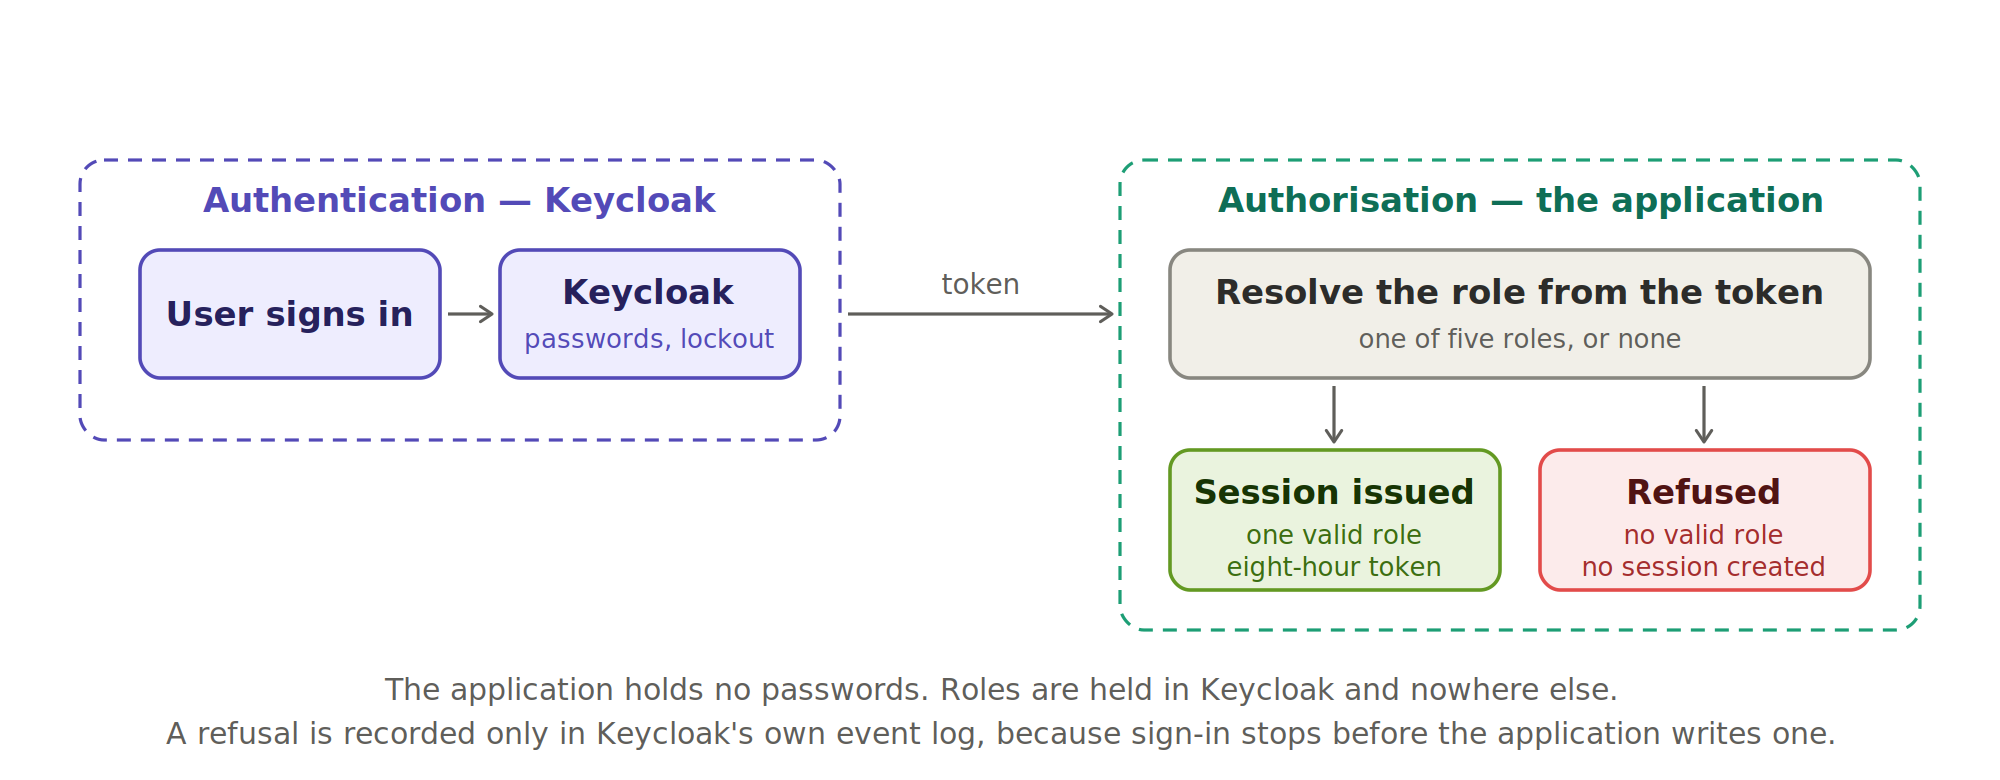
\includegraphics[width=0.95\textwidth]{figs/Figure4-Sign-In-Path.png}
  \caption{The sign-in path. Keycloak checks the password and returns a token carrying the user's identity and role. A token with one valid role gets a session; a token with none is refused.}
  \label{fig:signin-path}
\end{figure}

The server does not keep track of who is signed in. Instead, each user gets a token that proves who they are for eight hours, shortened from the library's default of thirty days. Because there is no server-side list, a token cannot be cancelled early; it stays valid until it expires. Keycloak also keeps its own separate session, timing out after twenty minutes of no activity or eight hours in total. The application adds a further twenty-minute idle timer of its own, with a one-minute warning. This one only runs in the browser: it is a visual timer, not something the server checks. It only catches someone who leaves the tab open and walks away. If the tab is closed instead, even briefly, the timer forgets that time passed and starts again from zero the next time the tab opens. So closing the tab does not stop a different person from opening the browser soon after and landing straight in. The timer also has no effect on the token's own eight-hour lifespan.

Two problems with this design have since been fixed. First, signing out now properly ends both sessions instead of just the application's. Before this fix, the next person on a shared computer could still be signed in as the last user, because only the application's side was cleared. Second, the two systems' timers were brought into line, so neither outlasts the other.

One limitation remains. Because there is no server-side session record, nobody can cancel a token early, and idle time cannot be enforced by the server. A disabled account is no longer part of this problem, since that is now checked directly on every request, described in the next section. But a genuinely stolen token would still work for the rest of its eight hours, since there is still no way to cancel it early.

\subsection{Account Status and AD Federation}

Keycloak originally held its own standalone accounts, created and managed only inside Keycloak itself, separate from any hospital system. During this work, Keycloak was connected to the hospital's own Active Directory through user federation instead (Section \ref{sec:met-tools} describes this decision). Accounts and their enabled or disabled status now come from AD, so a person's access in this system follows the same account AD already manages for them, rather than a separate copy Keycloak held on its own. A background job polls Keycloak every sixty seconds and mirrors its enabled/disabled state into the application's own database; every request checks that mirrored flag, which is what makes the check fast and consistent across every entry point, at the cost of a real but small window, typically under a minute, between a change in Keycloak and the application noticing it.

Access now requires two conditions to hold at once: the account must be enabled in Keycloak, and it must be enabled in the application's own record. The check is centralised in a single function that every entry point calls, so the six surfaces that enforce it (the sign-in check, three separate authorisation helpers used across the application's API routes, the page-level guard that runs on server-rendered navigation, and a client-side watcher that catches cached navigation those other checks do not see) can never disagree with one another. The two conditions are not symmetric. A Keycloak-side disable overrides everything: if Keycloak reports the account disabled, the user is locked out regardless of what the application's own record says, and no administrator can override that from inside the application. An administrator can still enable or disable an account independently through the application's own screen, and that setting is enforced on its own terms whenever Keycloak's side says enabled: an application-side disable still blocks the user even though Keycloak allows them. So the rule is closer to a logical AND than an override: both sides must say enabled, but only one side, Keycloak, can force a lock-out the other side cannot undo. A further condition covers users who disappear from Keycloak or AD entirely rather than being explicitly disabled: such an account is marked disabled in the application with a distinct ``not found'' status, and if that person's account later reappears, they are issued a new account rather than having the old one reactivated, a decision made jointly with the hospital's IT team since silently relinking an old account to a returning identity was judged a greater risk than the inconvenience of starting fresh.

\begin{figure}[H]
  \centering
  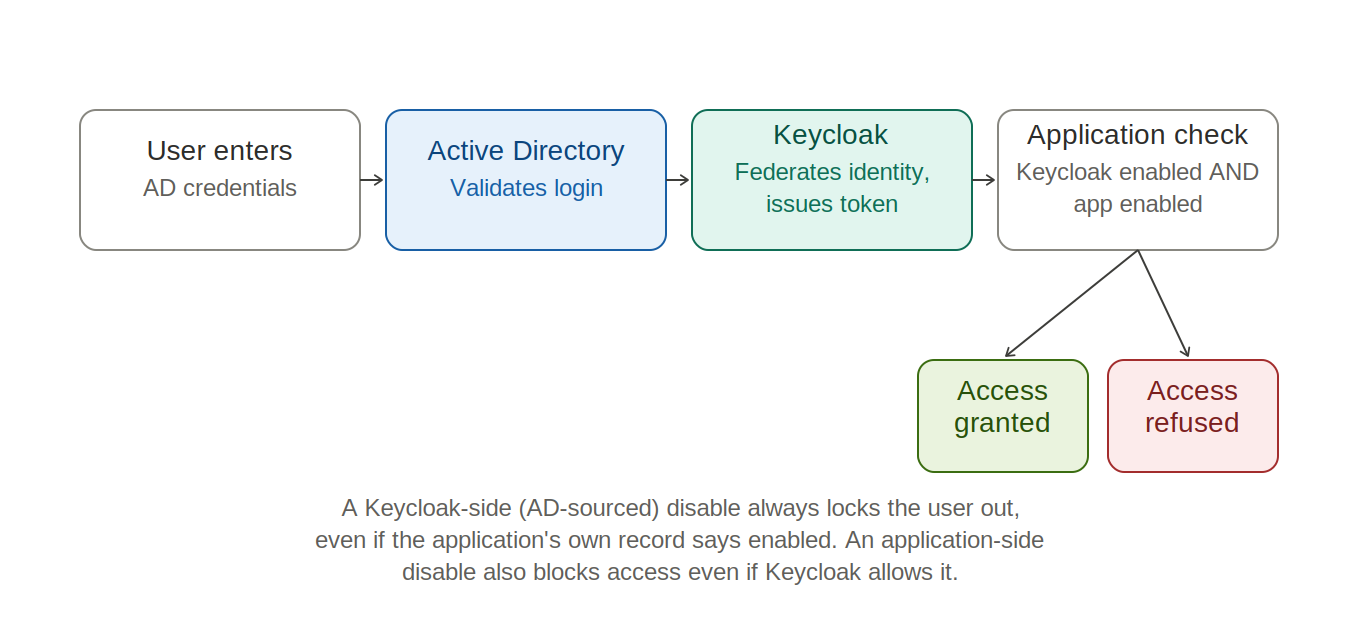
\includegraphics[width=0.95\textwidth]{figs/Figure5-Account-Status-AD-Federation.png}
  \caption{Account status after AD federation. Access requires two conditions to hold at once, checked on every request: the account must be enabled in Keycloak, whose status is itself now sourced from AD through federation, and enabled in the application's own record.}
  \label{fig:account-status}
\end{figure}

This design replaced an earlier approach that never worked. The original plan was a scheduled job: check each user's status against Keycloak on a timer, and disable anyone Keycloak reported as disabled. That job never actually ran, not even once. Its trigger was written to start on a hosting platform this deployment does not use, so nothing ever told it to run, and this was recorded as an open gap.

This is a real improvement over the original job. The original job never ran at all; this one runs reliably every sixty seconds. So the window a disabled account could still be used shrank from indefinite to roughly a minute, though it does not close the gap completely.

Two small limits remain, and neither is a flaw unique to this design. First, the check does not end an already-open browser tab the instant an account is disabled, and a request already in progress at the exact moment the flag flips still completes. This is true of any periodically-synced check. But the user's very next request after that, whether loading a new page or saving a form, is rejected before anything is written, with an ``account disabled'' response, and that refusal is logged. Second, anything the user genuinely did before that point stays correctly recorded; disabling their account part-way through a session does not change what already happened.

The other two background jobs, described in Section \ref{sec:impl-deployment}, are unrelated to account status and were not part of this change; their own outcomes are described there.

The two places used to record changes unevenly. A change made on the application's own screen was written to the audit trail. A change made directly in Keycloak or AD was not, so checking an account's history meant looking in two separate places. This has since been fixed: the same background job that copies a Keycloak-side disable into the application's database now also writes an audit entry at that same moment, so nothing extra is needed to record a Keycloak-side change.

One finding here turned out to matter more than it first looked. The session carries the ID Keycloak issues, but the application's own database uses a different ID for the same people. A check meant to confirm whether a case belonged to a particular doctor was comparing these two different IDs directly, and since they never match, doctors could not open their own cases. This showed up as several separate-looking problems at first: a list showing other people's drafts, a saved draft that opened read-only, and errors when saving. All of them turned out to share the same cause. This was fixed by converting one ID to the other before comparing them.

\section{Access Control Model}
\label{sec:impl-access-model}

Access control in this system combines the two models described in Chapter \ref{chap:lr}. Roles carry the decisions that follow a person's job, attributes carry the decisions that depend on a particular case, and the case's position in the workflow carries the decisions that depend on how far the work has progressed.

Mapped onto the four inputs NIST describes \cite{nist80162}, the model uses three of them. Subject attributes are the user's role, taken from the Keycloak token, and whether their account is active. Object attributes are the identifiers of the doctors assigned to a case and the step that case has reached. The rules are the forty-two action rules described below. Environment conditions are not used: no decision in this system depends on the time of day, the location of the request, or the network it arrives from.

\begin{table}[H]
\centering
\caption{The five roles and what each is responsible for.}
\label{tab:roles}
\begin{tabular}{|p{4.5cm}|p{9.4cm}|}
\hline
\textbf{Role} & \textbf{Responsible for} \\
\hline
Surgeon & Creating a case, entering the clinical description and their own fee \\
\hline
Anaesthetist & Taking an unassigned case from the pool and adding their assessment \\
\hline
Surgical Coordinator & Monitoring progress, and setting case priority \\
\hline
Finance & Building and confirming the cost, submitting the case, recording patient consent, finalising it, reviewing and sending the request to the insurer, and recording the insurer's answer \\
\hline
System Administrator & Managing user accounts, reading the audit trail, viewing all cases and patient data, assigning doctors to cases, and using emergency override powers (releasing a stuck case, removing documents) \\
\hline
\end{tabular}
\end{table}

Forty-two actions are defined across the system, and each has a rule saying which roles may perform it and under what conditions. They fall into four groups: eleven for the case lifecycle, six for finance and the insurer, six for documents and notes, and nineteen for reports, administration and reference data. The rules are kept in a separate document, updated as the code changes. It reached its third version during this work, each version following a round of checking.

The three factors work together, not separately. All three must hold, and if any one fails the action is refused. Take one question: may a surgeon edit this case? Using the role alone, the answer is yes, but that would let any surgeon edit any case. Adding assignment narrows it: yes, if the case is theirs. Adding the step narrows it again: yes, if the case is theirs and it has not yet reached Finance. Only the third answer is correct. The step is the least obvious of the three, because it changes the answer for a user who has done nothing: when the anaesthetist finishes their part, the case moves to Finance, and the surgeon becomes read-only. Figure \ref{fig:three-factors} shows the three factors as they are evaluated for one request.

\begin{figure}[H]
  \centering
  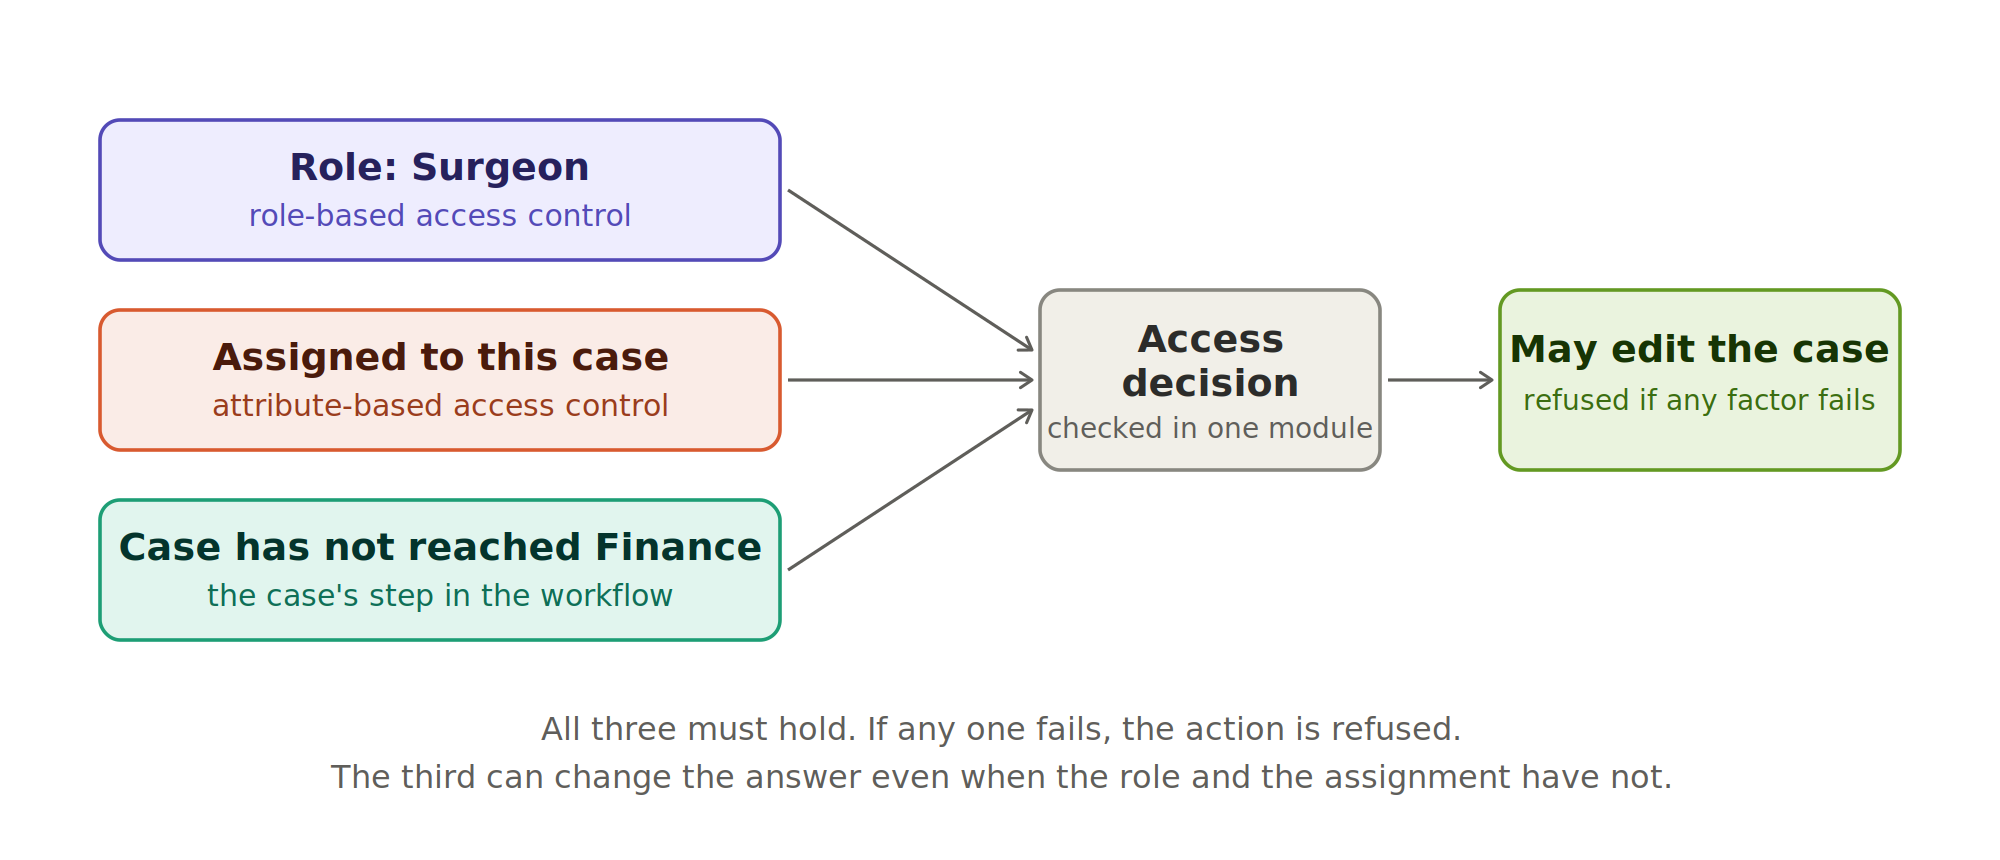
\includegraphics[width=0.95\textwidth]{figs/Figure6-Three-Factors-Decision.png}
  \caption{The three factors evaluated in every access decision. All three must hold; if any one fails, the action is refused.}
  \label{fig:three-factors}
\end{figure}

Underneath these rules is a split the hospital already used on paper. The doctors say what treatment is needed and what their own fee is. Finance builds the final price from that, adding or removing items as the case requires, and commits the hospital to the total. Neither does the other's job: a doctor cannot set what the hospital charges, and Finance does not decide what treatment is given. The case's step is what keeps them apart in software. Without it, a doctor could change a figure after Finance had already settled the price.

The Surgical Coordinator monitors progress and sets case priority; no role holds an edit right over another role's part of a case. The same separation applies to what leaves the hospital; Finance reviews a case before the request is sent, so nothing reaches an insurer without a person having checked it.

Assignment itself needed a rule of its own for the Anaesthetist role. Early on, opening an unassigned case made it the anaesthetist's immediately, with no typing and no saving required, and there was no way to hand it back if it had been opened by mistake. A case is now taken only when the anaesthetist saves or verifies it, and they can release it while it is still a draft. This matters for the same reason the case's step matters elsewhere: an action with a real consequence, becoming responsible for a case, was previously happening as a side effect of merely looking at something.

Access is decided in one place. A single module checks that the user has a session, that their account is active, and that their role is valid. Where the action needs it, the same module also checks that the case is theirs and has reached the right step. Nearly every address in the system calls it. Not every part uses the full check, though: at least eight places ask only whether the role is right, then work out for themselves whether the case belongs to the user, using their own separate copy of that rule rather than the shared one. This has already caused a real problem once, not just a theoretical risk: one of those copies fell out of step with the shared rule and briefly let a surgeon reach a case they should not have been able to see, before it was found and corrected. The other copies currently still agree with the shared rule, kept in sync only by developers remembering to update every copy by hand. Chapter \ref{chap:result} returns to this.

\section{Audit Logging}
\label{sec:impl-audit}

The audit log records every action that changes a case. An entry holds who acted, the role they held at the time, which case was affected, what was done, when, and which part of the system was used. Refused attempts are recorded too, with the reason. The entry does not record the device or the network address, so it can show that an account acted but not which machine was used.

The record is append-only: entries can be added, but never changed or deleted. This is enforced at the database level, through a trigger that rejects any update, delete, or truncate against the table outright, combined with a permission grant that removes the application's own database login's ability to attempt those operations at all. Neither the System Administrator role inside the application, nor a compromised application process using its normal database credentials, can alter a log entry; both are blocked before the operation would even reach the trigger. OWASP recommends exactly this for records that need to be trusted \cite{owasp2021}. It is what makes the log usable as evidence, rather than just something to look things up in.

One honest caveat sits underneath this, distinct from anything reachable through the application: whoever holds the database's own superuser credentials (a different, infrastructure-level actor entirely from any role the application defines) can disable the trigger with an explicit administrative command before modifying rows, then re-enable it. This is not a gap in the design so much as an inherent property of database superuser access generally, and it requires credentials no application role has access to. It happened exactly once, in a local development database, as an authorised, one-off cleanup of test data, carried out as a deliberate and distinct action rather than an ordinary delete, and never applied to the deployed system. Those credentials were handed over to the hospital at the end of the placement; the development team retains no database access on the live system. In short, the immutability guarantee described above is an application-level guarantee, holding against every role the application defines; who controls the database's own infrastructure-level superuser credentials is a separate governance question entirely, answered by who holds server access, not by anything this application can enforce in code.

The log saves a person's exact role at the moment they act, rather than looking it up again later. This fixes a real bug found during the work: Finance and the Coordinator had both been logged under the same generic label, STAFF, so old entries could not show which of the two had actually acted. Saving the exact role at the time also means that if someone's role changes later, old entries still correctly show what their role was back when they acted.

The administration screen presents a second log alongside it, and the two are not the same thing. The audit log records workflow events, as described above. The activity log instead records every successful request that passes the access checks, including the request body itself.

Two problems with this log have since been fixed. First, it had none of the protection the audit log has: rows could be changed or deleted, and no retention period was set. This is now fixed, and the activity log is in fact stricter than the audit log: the audit log's trigger allows one narrow exception (deleting a case correctly clears that entry's case reference), while the activity log has no such exception at all, so its trigger rejects every update, delete, and truncate outright.

Second, because the request body includes patient and clinical fields, those details used to be stored in the clear as a side effect of simply recording traffic. This is also now fixed: those fields are redacted before the row is written, replaced with a fixed marker instead of the real value. One small gap remains: a few fields, such as city, country, and gender, are not yet on that redaction list, so they would still be stored in full if a request happened to carry them. This is recorded as an open item in Section \ref{sec:conc-future}.

Two limits remain. Neither is a fault in the sense of a broken control; the second is a genuine, unresolved inconsistency worth stating precisely. The first is names, and it is more mixed than a single description covers. The audit entry's actor field is a reference to the user, resolved to a display name only when the record is read, so a later change to that person's name changes how every past entry involving them is shown. Separately, many entries also embed a name as literal text inside their own detail, ``Case finalised by John Tan (SURGEON),'' for instance, captured at the moment the action happened, and this text is genuinely frozen: it is written once into the append-only log and the database itself rejects any later change to it. The result is that a single entry can show two different names for the same person if they are renamed in between: the frozen name in the detailed text, and the current name in the actor field next to it, disagreeing with each other on the same row. Users can no longer rename themselves through the application, though an administrator creating or renaming an account, and a later sync that pulls a person's display name from Keycloak on each sign-in, can both still change it this way, so the inconsistency remains reachable. The same current-name behaviour reaches insurer emails, printed forms and the coordinator export, so a rename can also affect documents that have already left the hospital, independent of the log itself. The second limit is who may read the log. Administrators open it through the administration screen built as part of this work, and their own actions appear in both logs, so they can see what has been recorded about them. Separating those two responsibilities would mean redesigning who can read what, not fixing a fault.

Four things are not written down. A refusal that means only ``not yet'' (submitting a case before it is ready, or deleting one that has moved past draft) comes from the workflow rather than from a permission check, and only permission refusals are written down. A request for a case that does not exist is refused silently. A refused sign-in is recorded nowhere in the application, because sign-in stops before anything is written, so those attempts exist only in Keycloak's log. And nothing at all can be written when the database itself is down.

Nothing checks the log as it fills, and nobody reviews it on a schedule. Refused attempts are written down correctly, but no one is told, so twenty attempts in a row would sit in the table until somebody happened to open it. OWASP renamed this category in 2025 to include alerting for that reason \cite{owasp2025}. Both are recorded in Section \ref{sec:conc-future}: the software that would raise an alert, and the hospital routine that would review the records.

\section{Deployment}
\label{sec:impl-deployment}

My teammate deployed the application, and the hospital's IT department provided the server. What follows is about the security of that environment: what I found in its configuration, what was corrected, and what is still open.

The system runs on a Windows server the hospital owns, reachable only from inside the hospital. Four programs run on it side by side: the application, the database, Keycloak, and the FHIR server. None of them can be reached from the internet.

Among the four, the database and the FHIR server are the most locked down: only the machine itself can reach them, nothing else. Keycloak is the one deliberate exception. It can be reached from elsewhere on the hospital's internal network, though still never from the internet, because a person's browser needs to talk to Keycloak directly during sign-in.

Patient data is read from the hospital's own system, with limited read-only access granted by the IT department. This deployment does not own or hold the primary patient record; ANZER remains the single source of truth for that data, as Section \ref{sec:met-tools} states.

That said, patient information can still end up inside this system's own storage in one place. As Section \ref{sec:impl-audit} describes, the activity log records the body of every successful request, and some of those requests carry patient identifiers and clinical detail. That information used to be stored as-is, as a side effect of logging traffic. It is now redacted before the row is written, though a small number of fields are not yet covered, recorded as an open item in Section \ref{sec:conc-future}.

The application has a shortcut for developers: skip sign-in, pick a role, no password. It is useful on a laptop and dangerous on a server. The template that people copy when setting up a new server had that shortcut switched on, so anyone following it would have built a server that anyone could walk into. This was fixed twice. The template now has it switched off, and the application refuses to start if the shortcut is on in production.

The browser-facing connection now runs over HTTPS. Two internal connections remain unencrypted: Keycloak to the application, and Keycloak to Active Directory, so credentials and status information passing over those two links still cross the network in the clear. Keycloak also cannot leave its development mode until its own connections are encrypted. Whether the database's disk is encrypted has not been confirmed either way. On a Windows server, that would mean turning on BitLocker, which is a setting on the server itself, not something this application configures, so it is a decision for the server administrator to make.

The four containers are third-party software, so rather than assume they were safe I scanned them, and Chapter \ref{chap:result} reports what that found. One problem was found without a scanner. Keycloak had not been told where to keep its accounts, so it had defaulted to H2, the lightweight, file-based database built into Keycloak itself, meant only for local testing and explicitly not recommended by its makers for a real deployment. H2 stores its data as a single file inside the Keycloak container rather than as a separate, durable service, so losing that container would have meant losing every account outright, and the file could not be backed up without shutting Keycloak down first to release it. Keycloak was reconfigured to use the PostgreSQL database already running alongside it instead, in a separate schema with its own restricted login, so accounts now live in the same durable, backed-up database as the rest of the system rather than a throwaway file tied to one container's lifetime.

Three background jobs existed at the time this was written. One was meant to disable an account when Keycloak said it should be disabled, described in Section \ref{sec:impl-iam}. Another was meant to warn staff when a case was taking too long. A third was meant to close cases automatically once they passed a deadline.

None of the three ever ran, and all three failed for the same reason: their schedule was written in a format meant for a specific cloud hosting service, one this project does not use. The hospital's own server had no way to read that format, so nothing ever told these jobs to start.

One of the three also had a second, separate way it was supposed to run, triggered from the browser whenever the application was open. This did not work either: it used the wrong technical method to make the request, so the server rejected it immediately, before the job itself ever ran.

Each of the three broken jobs has since taken a different path. The account-disable job was not fixed directly; it was replaced entirely by the periodic dual-check design described in Section \ref{sec:impl-iam}. The deadline-closure job was removed outright, a deliberate decision rather than a fix: it used to close cases after a flat 30-day window, unrelated to the SLA tiers described below, and before deletion, a database check confirmed it had never actually closed a single case in the system's history. The slow-case warning job was kept and given a real trigger, but not the one originally planned: instead of an OS-level scheduler like Windows Task Scheduler, it now runs on a timer inside the application itself, firing every 15 minutes while the application is running, a real fix, but a weaker guarantee than an OS-level schedule, since this timer stops if the application process stops.

The rule the slow-case warning job checks against was also revised after this was first written. Cases originally fell into two service-level categories, adjustable from a settings screen. This was changed to three fixed categories: Emergency (1 hour), Urgent (8 hours), and Routine (48 hours). Each number is a threshold, the number of hours a case may wait before it counts as overdue for that category, read from a database-backed configuration rather than the earlier hardcoded pair. The permission to change these three thresholds was built for the Surgical Coordinator and System Administrator roles, with validation, a database write, and its own audit entry, and this was tested working.

This is a different thing from changing an individual case's own category, which is a separate, everyday action the Coordinator still performs normally, described in Section \ref{sec:impl-access-model}; what is disabled here is only the ability to edit the three threshold numbers themselves. This ability to change the thresholds is not usable today. Both the screen that edits them and the route behind it are switched off, deliberately, behind a single flag. This was done after testing found two real bugs in the editor: a saved total that was written but never read anywhere, and a dashboard countdown that used a separate table the editor did not update. Rather than ship a partially working editor, both the screen and the route were locked pending a decision. The route also refuses every request outright, no matter who is asking, so a disabled feature can never be mistaken in the logs for someone being refused because of their role.

Reading the current thresholds still works for everyone. Only changing them is switched off. So in practice, the thresholds are fixed for every role today, though not because that was the design. The ability to adjust them exists, and has been built and tested; it is simply waiting on that flag to be turned on.

This job does not wait until the deadline to raise a warning. Instead, it raises its warning in stages as a case approaches each threshold. The warning itself only shows up inside the application, as a status or a flag; it is not sent out as an email.

These three tiers apply only to this warning job. They do not apply to the separate deadline-closure feature described earlier. That feature used its own unrelated rule, a flat 30-day window, and was removed entirely rather than being connected to this newer, tiered system.

\chapter{Result and Discussion}
\label{chap:result}
\chaptermark{Result and Discussion}

This chapter reports what the security work produced, and what those results mean. Section \ref{sec:result-result} gives the findings from both checking methods, the numbers each produced, and the decisions taken on them. Section \ref{sec:result-discussion} looks more closely at two of those results: how permissions in this system depend on more than the user's role, and why the automated tools did not find the problems that manual testing found.

\section{Result}
\label{sec:result-result}

\subsection{How the System Was Checked}

The system was checked in two ways. Automated tools looked at three things: the outside packages the system uses, the container images it runs in, and the project's own code. Manual testing was done role by role on the running system, using one account for each role and following each case from creation to the insurer's decision. Both were done in the same period, on the same version of the system, and the rules being tested covered forty-one actions across five roles.

Two checks were still to come. The hospital's IT Security Division had not yet tried to break into the system, and the container settings had not yet been checked against the CIS Docker Benchmark. Neither had been done when this was written.

\subsection{Package and Container Scanning}

\begin{table}[H]
\centering
\caption{Scanning targets and findings.}
\label{tab:scan-targets}
\begin{tabular}{p{3.6cm}p{2.6cm}p{6.8cm}}
\toprule
\textbf{Target} & \textbf{Tool} & \textbf{Findings} \\
\midrule
npm packages & npm audit & 15: 2 critical, 4 high, 8 moderate, 1 low \\
Keycloak 26.6.4 & Trivy & 16 high, 0 critical \\
PostgreSQL 16 & Trivy & 72, then 55 after an update \\
HAPI FHIR 7.4.0 & Trivy & 132: 27 critical, 105 high \\
Repository and files & secretlint & No secrets found \\
\bottomrule
\end{tabular}
\end{table}

Every problem was in software the project uses rather than in code the team wrote, other people's libraries and container images. Updating the login library cleared both critical findings, taking the count from 15 to 13 with none critical. Eight of the remaining problems were in the application framework, and looked at first as though they needed a major upgrade. They did not: moving from version 15.5.20 to 15.5.22 was enough. One package, sharp, is still below the version its advisory asks for, because the fix offered would have undone the framework update. That was judged a step backwards, and it is recorded as an open item.

Updating the database image reduced its findings from 72 to 55, and its critical findings from 19 to 17; the rest have no fix available yet, so nothing can be installed. The FHIR server image was the worst of the three, and whether it is needed at all was raised as an open question for the team rather than treated as something to patch. Keycloak was also found to be keeping every account in its own built-in database, which its makers say not to use for real systems. It was reconfigured to use the PostgreSQL database already running alongside it, in a separate area with its own restricted login. The accounts on my own machine moved across keeping their original identifiers; any other installation starts with an empty Keycloak and needs its accounts created again.

\subsection{Checking the Project's Own Code}

CodeQL was planned for this step, but GitHub offers it free only on public repositories and a private one needs a paid licence. Semgrep was used instead, covering the same kinds of checks. It applied 257 rules across 356 files and returned 15 findings.

\begin{table}[H]
\centering
\caption{What Semgrep found.}
\label{tab:semgrep}
\begin{tabular}{p{8.5cm}p{2cm}}
\toprule
\textbf{Type} & \textbf{Count} \\
\midrule
Path traversal, looked at separately & 1 \\
Regular expression built at run time & 3 \\
Unsafe text in log messages & 5 \\
Unpinned action versions & 4 \\
Installer piped into a shell & 1 \\
Package setting & 1 \\
\bottomrule
\end{tabular}
\end{table}

None of the common problems appeared. There was no SQL injection, no cross-site scripting, no password left in the code, and no way around the login. Nothing was about access control.

The path traversal was looked at more closely and could not be used. The database check runs before any file is written, and an invalid case identifier fails there, so the write is never reached. That protection was accidental rather than planned, so it was recorded as something to make deliberate: check the identifier properly, and mark the order of steps as security-critical so a later change does not remove it by accident.

\subsection{Manual Role-by-Role Testing}

A finding was counted as access control if it changed which users could do which action in which case. Findings about audit logging, sessions, input checking, data quality, and screen behaviour were counted separately. The logout defect was counted as access control rather than as a session problem, because its effect was that one user reached another user's account without logging in. On this basis the security phase recorded 47 findings, of which 23 were about access control.

\begin{table}[H]
\centering
\caption{The 47 findings by type.}
\label{tab:findings-by-type}
\begin{tabular}{p{8.5cm}p{2cm}}
\toprule
\textbf{Type} & \textbf{Count} \\
\midrule
\textbf{Access control} & \textbf{23} \\
Screens, data quality, workflow & 16 \\
Audit and logging & 4 \\
Input checking & 1 \\
Sessions & 1 \\
Deployment and configuration & 1 \\
Closed, not a defect & 1 \\
\bottomrule
\end{tabular}
\end{table}

The 23 access-control findings fell into six groups.

\begin{longtable}{p{3.6cm}p{9.3cm}}
\caption{The six kinds of access-control finding.}
\label{tab:six-kinds} \\
\toprule
\textbf{Group} & \textbf{Example} \\
\midrule
\endfirsthead
\multicolumn{2}{@{}l}{\textbf{Table \thetable} \ldots continued} \\
\toprule
\textbf{Group} & \textbf{Example} \\
\midrule
\endhead
\midrule
\multicolumn{2}{r}{\textit{Continued on next page}} \\
\endfoot
\bottomrule
\endlastfoot
Seeing cases they should not & A surgeon's list showed other surgeons' drafts \\
Actions held by the wrong role & Submit and finalise sat with the Coordinator, and refused Finance, the role that owns them \\
No lock on the case's step & Doctors could still edit details and costs after Finance had reviewed the case \\
Wrong identifier compared & Assignment checks compared two different kinds of user id, so doctors could not reach their own cases \\
Letting people through on failure & The disabled-account check allowed access when it found no record \\
Sessions outliving logout & Logging out left the Keycloak session open, so the next person at a shared computer entered the previous user's account \\
\end{longtable}

\subsection{Fixed and Left for Later}

Most findings were fixed before deployment. Twenty-four improvements were recorded as decisions to leave for later, each with a stated reason and an owner.

\begin{longtable}{p{4.4cm}p{8.5cm}}
\caption{Examples of work left for later, and why.}
\label{tab:left-for-later} \\
\toprule
\textbf{Left for later} & \textbf{Reason} \\
\midrule
\endfirsthead
\multicolumn{2}{@{}l}{\textbf{Table \thetable} \ldots continued} \\
\toprule
\textbf{Left for later} & \textbf{Reason} \\
\midrule
\endhead
\midrule
\multicolumn{2}{r}{\textit{Continued on next page}} \\
\endfoot
\bottomrule
\endlastfoot
Coordinator pricing fields stay unlocked & A deliberate safety valve. The team agrees changes in person, and the log records who edited \\
Case deadline feature & Dropped from this phase. It is already inactive, since nothing on the server starts that job \\
Duplicate drafts & Needs screen buttons that do not exist yet \\
Appeal improvements & There is no button to start an appeal, and an appeal makes the doctors start again \\
Refused sign-ins not recorded in the application log & Sign-in stops before the audit write; the attempts exist in Keycloak's log \\
A refused user cannot switch accounts & No session is created, so signing out cannot end the identity provider's session \\
\end{longtable}

\subsection{Findings Worth Describing}

The file holding the page rules sat at the top of the repository, while the application runs from a folder inside it. The framework only looks inside that folder, so it never found the file, and those rules had never run at all. Nothing was exposed, because the central module was checking every request anyway. It was left as it stood: switching on a gate that has never run means every page might behave differently, and that needs a full test pass across the whole system.

A related finding was fixed at once. A user who belonged to no group still received a working session, and could reach any page and any address that only asked whether someone was signed in, including a case list that returned every case. Sign-in is now refused when no valid role is found.

Two findings concerned the point at which work should stop, and both were fixed. Doctors could change the diagnosis and the cost after Finance had reviewed the case, without Finance knowing, so Finance had committed to a figure the case no longer matched. Editing now stops the moment a case reaches Finance. This is the finding that shows the case's step has to be part of the rule: the doctor's role has not changed, and the case is still theirs, but the answer must change anyway. Separately, opening an unassigned case made it yours immediately, with no typing and no saving, and there was no way to hand it back. A case is now taken only when the anaesthetist saves or verifies it, and they can release it while it is still a draft.

Logging out cleared only the application's own session while the Keycloak session stayed open, so the next person at a shared computer entered the previous user's account with no password. Signing out now ends both.

The log had a gap too: it was written only after a successful action, so a refused attempt left nothing behind. This was partly closed. Refusals where someone reaches for a case that is not theirs are now recorded, with the person, their role, the case and the reason. Refusals that only mean ``not yet'' are still not recorded, and neither is a deletion refused because the case has moved past draft.

A further gap sits earlier. When someone with a real account but no role is refused at sign-in, nothing is written to the application's log at all, no success, no failure, because sign-in stops before the point where anything is recorded. Those attempts appear only in Keycloak's own log, which is switched on, so an investigation has to look in two places rather than one.

Two further weaknesses concern the audit trail itself. Records hold a reference to the user rather than the name as it stood at the time, and look the name up when the record is read, so a rename relabels every past entry for that person, including sign-ins and refused attempts. The same name reaches insurer emails, printed forms and the coordinator export, so a rename would also change documents that had already left the hospital. The path that made this reachable was closed, but the design is unchanged. Separately, administrators can open the audit trail while their own actions are recorded in it, so a privileged user can see what was captured about them. Both are design changes rather than fixes, and both are recorded for later. Neither would be found by a scanner, and role-by-role testing did not flag them either, because the system behaves exactly as it was built to.

Two findings concerned patient data, and neither has been resolved. Removing a patient identifier from the screen did not remove it from the data sent to the browser, where the identifier, the national ID and the phone number were still readable. Fixing this properly means sending only what each row needs and moving the search to the server, which was judged too large a change before go-live.

The second concerned transport. The system runs over plain HTTP, which the browser reports directly: it shows the connection as not secure. Patient data and session cookies therefore cross the hospital network in the clear, and the strict-transport header has no effect without encryption. This is also a departure from a standard the project otherwise follows, since FHIR's security guidance states that production data should be sent over an encrypted connection \cite{hl7fhir}. Enabling encryption is a server or proxy configuration rather than an application change, and it is the most important item to resolve before the system carries real patient records.

Two further findings came to light during the final review, after the counts above were settled. The first concerns a second log. Alongside the audit trail, the system keeps an activity log of every successful request, including the request body, so it accumulates patient identifiers and clinical detail as a side effect of recording traffic. The audit trail is append-only, enforced by the database. The activity log has no such protection: its rows can be changed or deleted, and no retention period is set. Both logs need that protection, and only one has it.

The second concerns the background jobs. Three exist, and none has ever run. All three declare their schedule in a file meant for a hosting service the project does not use, and nothing on the deployment server starts them. One of the three is the job that disables accounts Keycloak reports as disabled, so the gap it was written to close is still open in practice.

\subsection{OWASP Top Ten Assessment}

Every category of the OWASP Top 10:2021 was rated against evidence from this project. Categories were rated strong where the risk was assessed and no significant gap remains, partial where controls exist but a known gap is recorded, and needs work where a material weakness is unresolved.

\begin{table}[H]
\centering
\caption{OWASP Top 10:2021 ratings.}
\label{tab:owasp-ratings}
\begin{tabular}{p{2cm}p{10cm}}
\toprule
\textbf{Rating} & \textbf{Categories} \\
\midrule
Strong & A01 access control, A06 outdated components, A07 authentication \\
Partial & A02 cryptography, A03 injection, A04 design, A05 misconfiguration, A08 data integrity, A09 logging, A10 request forgery \\
Needs work & --- \\
\bottomrule
\end{tabular}
\end{table}

No category was rated as needing work, though three of the partial ratings hold the largest open items. A02 covers encryption in transit and at rest: the system runs over plain HTTP, nobody checks whether the disk is encrypted, and the header telling browsers to insist on encryption does nothing until encryption is on. A05 covers the identity provider running a version past its end of life, an out-of-date FHIR server image, and Keycloak running in its development mode. That last one cannot be fixed on its own, because production mode will not start without encryption, so it waits on the same decision as A02. A fourth A05 item was fixed during the phase: Keycloak's built-in database, which was replaced by the PostgreSQL database already running alongside it.

A09 rests on an audit trail that cannot be changed or deleted, protected by the database itself, and that records refusals along with the reason. Against that sit three gaps: nothing watches the log as it fills, the activity log holds request bodies without the same protection, and the jobs meant to run on a schedule never run. The rating is partial because real controls exist and every gap is recorded, but the activity log is the one that would most change this assessment if it stays as it is.

Two of the strong ratings still have something recorded against them. A06 rests on scanning and fixing packages and container images, but two remain out of date because no fix exists yet, and both are carried into Section \ref{sec:conc-future}. A07 relies on Keycloak, the password rules, account lockout and session handling, but there is no multi-factor authentication, which was deliberately left to a later phase.

A01 was rated strong. It is also the one category no scanner could assess, it was closed by the role-by-role testing described above.

\section{Discussion}
\label{sec:result-discussion}

\subsection{Permission Depends on More Than the Role}

Role-based access control asks one question: what is this user's role? In this system that was never enough on its own. Every rule rested on three things together, and removing any one of them gave the wrong answer.

\begin{table}[H]
\centering
\caption{The three factors, with an example of each.}
\label{tab:three-factors-table}
\begin{tabular}{p{2.6cm}p{9.4cm}}
\toprule
\textbf{Factor} & \textbf{Example from this system} \\
\midrule
Role & Only a surgeon may create a case \\
Assignment & A surgeon sees only their own cases; a doctor may remove only files they uploaded \\
The case's step & Once a case reaches Finance, both doctors become read-only \\
\bottomrule
\end{tabular}
\end{table}

The third factor is the easiest to miss, because it changes the answer for a user whose role and assignment have not changed at all. A surgeon may edit their own case one day and not the next, not because anything about the surgeon changed, but because the anaesthetist has since finished their part and the case has moved to Finance. Neither the surgeon nor Finance did anything. A third person completing their work changed what the surgeon was allowed to do.

This was found as a real defect: doctors could change the diagnosis and the cost after the case had reached Finance, and Finance did not know.

That matters more than a single wrong permission, because it undoes a rule the hospital depends on. The doctors say what the treatment costs and Finance authorises it, and neither does both. If a doctor can change the figure after Finance has approved it, the separation exists on paper only. The case's step is what keeps the two apart.

The lock has a cost, and it was accepted knowingly. Once both doctors have verified, they are read-only. So if a correction is needed later, if the insurer asks for more clinical detail, for instance, the doctor cannot supply it directly, and the change has to go through Finance or the coordinator. Uploading a document stops at the same point. The team judged this acceptable for a first phase, because the alternative is letting clinical data change underneath a price Finance has already confirmed. Whether to loosen the lock, and how, was left until after the go-live test.

Permission in this system depended on three things together, and the case's step was the one most easily overlooked. Most of the twenty-three access-control findings turned on assignment or on the case's step, not on the role.

\subsection{Why the Scanners Found No Access-Control Problems}

Semgrep applied 257 rules to 356 files and returned 15 findings, none of them about access control. This is not a failure of the tool.

A rule in a scanner describes the shape of code. It can spot a query built by joining text together, or a password written into a file, because those look a particular way wherever they appear. ``A coordinator may not submit a case'' has no shape. It is a decision the hospital made about who is responsible for what, and nothing in the code marks it out from any other function call. A scanner cannot check a rule it was never given.

What this project adds is a measurement from a working clinical system. On the same code, in the same period, a general-purpose scanner found nothing in this category while role-by-role testing found twenty-three problems, several of them serious. Zhu and colleagues report the closest comparison: automatic analysis of six applications found a set of vulnerabilities, and when developers gave the tool the application's own access control rules, twenty more appeared that the automatic methods had missed \cite{zhu2015}.

A related gap appeared before any scanning was done. The access control rules were not written before the code, they were read out of it, because the code came first. Setting that description against the workflow the team needed showed that a substantial number of rules did not match what the hospital wanted, and that some expected actions did not exist at all. Sun, Xu and Su note that access control rules are specific to each application, which makes it hard to get a precise specification for a tool to enforce \cite{sun2011}. Here there was no specification to enforce against: it had to be recovered from the code first.

The consequence is short. A clean scan is evidence about code patterns. It is not evidence that the right people can do the right things, and it should never be recorded as though it were.

\subsection{Layered Checks, and the Guard That Never Ran}

The clearest illustration of layered checking came from a mistake. The file holding the page rules sat outside the folder the framework reads, so it never loaded, and that whole layer had been doing nothing for the life of the project. Nothing was exposed, because the central module was checking every request anyway. What only emerged later was that the file's own settings excluded those addresses entirely, so even had it loaded, it would never have guarded what it appeared to guard. It read as a control, and was never capable of being one.

Two things follow. Nobody knew the layer was dead until it was found by accident, which is an argument for testing that a control actually runs rather than assuming it does because the code exists. A protection that has never run offers nothing, and it looks exactly like a working one until someone checks. The system survived because the decision was made in one place, which is what OWASP asks for, that access control be implemented once and reused throughout an application \cite{owasp2021}. That is not complete: some parts take the simpler check and then work out the assignment rule again in their own code, so the same rule sits in two places. Rules in two places drift apart, and this is recorded in Section \ref{sec:conc-future}.

The same pattern appeared twice more. In the path traversal finding, an attack failed only because a database check happened to run first, the system was safe, but not for the reason anyone had designed, and changing the order of steps later would have removed that protection without warning. And three background jobs are written, correct, and have never run: nothing on the deployment server starts them, and the one call that does reach a job uses a method the route does not accept, so it is rejected before anything executes. One of the three is the job meant to close the gap left by a session that cannot be withdrawn. The control exists, and the gap is still open.

\subsection{What This Suggests for Similar Systems}

Three points carry beyond this project.

Where a workflow hands responsibility from one group to another, the state of the work belongs in the permission rule alongside the role. Without it, the handover is not enforced at all.

Where authorisation rules come from an organisation rather than from the code, they have to be tested by using the system as each role, because no scanner has access to them.

And where a control matters, it is worth confirming that it runs. Code that exists and code that executes are not the same thing.

\chapter{Challenges, Conclusion and Future Work}
\label{chap:conclusion}
\chaptermark{Challenges, Conclusion and Future Work}

This chapter covers the difficulties encountered during the security work, the conclusions drawn from it, and the work that remains for later phases.

\section{Challenges}
\label{sec:conc-challenges}

\subsection{Technical Challenges}

\textbf{I started with no background and no map.} I had not built software before this project, so reading someone else's code and changing it safely were things I learned while doing them. Nor was there a structure to follow. At the beginning my learning was scattered, one topic, then another, in no order. What structure existed came later, from the frameworks in Chapter \ref{chap:met} and from asking the IT team, my mentor, my teammates and AI tooling.

\textbf{Security began after development.} A teammate wrote the application code first, because I was new to this area and the access rules were not ready, and the team could not wait. That was the right call for a six-month phase, but it set the method: I could not build access control from a written table, because the code already existed. I read the code, wrote down what it allowed each role to do, compared that against the workflow the team needed, and changed the code where they differed. A substantial number of rules did not match what the hospital wanted, and some expected actions did not exist at all.

\textbf{The domain was entirely new.} Electronic medical records, the hospital's own information system, the FHIR standard, and how insurance approval works were all unfamiliar. Before any of us could start building, we spent weeks understanding the process itself, what the hospital already had, what they wanted, and how people actually worked. Access control cannot be designed without understanding the workflow it protects, so learning the domain was a prerequisite rather than background reading.

\textbf{Evaluation used the time that implementation would have needed.} The team spent several months trialling Microsoft Entra ID before establishing that the hospital's requirement to host on its own servers ruled it out. Keycloak was then deployed and learned from the beginning. The hospital's staff directory was made available for federation later in the phase, but by then there was no time left to connect it. Federation is therefore understood and planned but not built, and it is recorded in Section \ref{sec:conc-future}.

\textbf{Almost everything was designed by revision.} Access rules were built one at a time, decided, implemented, checked, and sometimes the requirement itself changed once people saw the result. The audit trail had no template at all: I decided what to record, revised it, took it to the IT head, revised again, researched, and revised once more. Verification behaved the same way, since each time I finished checking, a teammate found something that sent the work back round. The gaps recorded in Chapter \ref{chap:result} reflect a design arrived at by iteration rather than one worked out in advance.

\textbf{Some problems appeared only after deployment, and signing in was the hardest of them.} Using an identity provider was new to everyone on the team, not only to me. Nobody had deployed one before, so each problem had to be worked out from first principles rather than looked up. Work that ran without trouble on my own machine failed once installed: sign-in stopped working, and staff on other machines could not sign in at all. The application's database also turned out to be empty, because one database update had failed partway and blocked every update after it. These reached me as reports from the deployment side rather than through my own testing, and my part was working out the cause of each.

\subsection{Stakeholder Challenges}

Nobody comes to you. At this workplace, if you need something you have to ask for it, and everyone whose knowledge I needed had their own work to do. Help was not continuously available. Learning to approach people directly, at the right moment, was a change in how I work, and it had to come before any of the technical work could proceed.

The workflow had to be understood before it could be secured. Who may do what depends on which step a case has reached, so the flow had to be settled before the rules enforcing it could be written. The flow follows the hospital's existing paper procedure, so I began with the paper, reading the forms, following how a file moved between departments, and learning the terms doctors and hospital staff use for what those forms contain. None of that vocabulary was familiar. The flow was not mine to settle either: the Coordinator and Finance teams had to agree to it between them, over a series of meetings, and each change to it changed the rules enforcing it.

Even now, with the flow decided and built, it is not certain that it matches what those teams expect in daily use.

Some findings were questions rather than defects. Whether the coordinator should keep the ability to change prices after Finance has confirmed them is a decision for the hospital, not for me, and so is whether the FHIR server is needed at all. These took longer to settle than code fixes. Changes of that kind also affected my teammates, locking a form or restricting an action alters what they are building against, so they were raised before being applied rather than afterwards.

\section{Conclusion}
\label{sec:conc-conclusion}

This project secured a system that automates the Guarantee of Payment process at a Cambodian hospital. An identity provider was deployed on the hospital's own servers, access control was built across forty-two defined actions for five roles, an append-only audit trail was added, and the result was checked by two methods before deployment.

The clearest result came from comparing those methods. Static analysis applied 257 rules across 356 files and returned fifteen findings, none about access control. Role-by-role testing of the same system in the same period produced forty-seven findings, twenty-three of them access control. The scanner was not badly configured: access rules here come from how the hospital divides responsibility, not from anything visible in the shape of the code, and a tool cannot check a rule it was never given.

The second result concerns what those rules depend on. A permission is decided by three things together, the user's role, whether the case is theirs, and how far the case has progressed. The third is easiest to miss, because it changes the answer for a user whose role and assignment have not changed: a surgeon becomes read-only when the anaesthetist finishes and the case moves to Finance. That step is what enforces in software the separation the hospital already practised on paper.

The limits are stated rather than implied. There is no automated test suite, so verification was manual and happened once. The system is served without encryption. The assessment is by the person who built the controls, not an independent audit. And the final review found controls that had never run at all, a page-rule file the framework never loaded, and three background jobs nothing on the server starts, which is the plainest evidence that a system checked once is not a system that stays checked.

What this project produced is therefore not a secure system but a documented one: rules that can be checked, a record of what was found, and a list of what remains with an owner against each item.

\section{Future Work}
\label{sec:conc-future}

Twenty-eight items remain. Some need access or authority I did not have, and some are commitments only the hospital can make. The rest were within reach but not reached before this was written, and some of those may be taken up in the remaining month of the placement.

\begin{longtable}{p{0.6cm}p{8.4cm}p{3.3cm}}
\caption{Work remaining, and who can carry it.}
\label{tab:future-work} \\
\toprule
 & \textbf{Item} & \textbf{Who can carry it} \\
\midrule
\endfirsthead
\multicolumn{3}{@{}l}{\textbf{Table \thetable} \ldots continued} \\
\toprule
 & \textbf{Item} & \textbf{Who can carry it} \\
\midrule
\endhead
\midrule
\multicolumn{3}{r}{\textit{Continued on next page}} \\
\endfoot
\bottomrule
\endlastfoot
\multicolumn{3}{@{}l}{\textbf{Server configuration}} \\
1 & Enable transport encryption, the most important item outstanding & Server administrator \\
2 & Confirm whether the server's disk is encrypted & Server administrator \\
3 & Confirm the server's clock is synchronised & Server administrator \\
4 & Schedule the three background jobs, none of which currently runs & Server administrator \\
5 & Assess availability and denial of service & Server administrator \\
6 & Review whether the server is powerful enough for real use & Hospital IT \\
\addlinespace
\multicolumn{3}{@{}l}{\textbf{Development in the next phase}} \\
7 & Record the device and network address in audit entries & Security \\
8 & Raise an alert on repeated refused attempts & Security \\
9 & Protect the activity log, or stop it recording request bodies & Security \\
10 & Add multi-factor authentication & Security \\
11 & Connect federation with the hospital's staff directory & Security \\
12 & Deploy the corrections verified locally & Development \\
13 & Hold session state on the server, so sessions can be withdrawn and differ by role & Security \\
\addlinespace
\multicolumn{3}{@{}l}{\textbf{Hospital governance}} \\
14 & Set an audit trail policy and a retention period & Hospital \\
15 & Review user access rights on a schedule & Hospital \\
16 & Review what administrators do & Hospital \\
17 & Collect logs centrally rather than leaving them in the application & Hospital \\
\addlinespace
\multicolumn{3}{@{}l}{\textbf{Design changes}} \\
18 & Separate administering the system from reading the audit trail & Team decision, then development \\
19 & Store names when a record is written rather than looking them up when read & Security \\
20 & Record refused sign-ins in the application's own log & Security \\
21 & Record account changes made in Keycloak & Security \\
22 & Remove the duplicated assignment rule, so it exists in one place & Security \\
23 & Check permission before checking whether a case exists & Security \\
24 & Build the role override control or remove it & Team decision \\
\addlinespace
\multicolumn{3}{@{}l}{\textbf{Outstanding assessment}} \\
25 & Pre-deployment assessment with the hospital's IT Security Division & IT Security Division \\
26 & Check the container settings against the CIS Docker Benchmark & Whoever assesses \\
27 & Re-assess against OWASP Top 10:2025, where Security Misconfiguration has moved from fifth place to second \cite{owasp2025} & Whoever assesses \\
28 & Pin tool versions, since neither scanner was pinned and the results cannot be reproduced exactly & Whoever repeats the scan \\
\end{longtable}

Three of these are connected. Encryption blocks two others: Keycloak cannot leave its development mode until it exists, and the disk check belongs to the same piece of work. The background jobs need scheduling because their schedule is declared in a file the deployment does not read, so none has ever run, including the one meant to close the session gap. And the activity log matters more than its position in the list suggests, because it holds patient data without the protection the audit trail has.

Of the twenty-eight, ten belong to the server administrator or the hospital rather than to the application.



%% REFERENCES
\printbibliography[heading=bibintoc,title={References}]

\end{document}

